% !TEX program = tectonic
\documentclass[a4paper,11pt]{article}

% ===================== Packages =====================
\usepackage{fontspec}
\usepackage[a4paper,top=2.8cm,bottom=2.8cm,left=2.6cm,right=2.6cm,headheight=15pt,headsep=10pt,footskip=22pt]{geometry}
\usepackage{array}
\usepackage{amsmath}
\usepackage{amssymb}
\usepackage{booktabs}
\usepackage{tabularx}
\usepackage{longtable}
\usepackage{enumitem}
\usepackage{xcolor}
\usepackage{setspace}
\usepackage{titlesec}
\usepackage{titletoc}
\usepackage{float}
\usepackage{placeins}
\usepackage{tikz}
\usepackage{fancyhdr}
\usepackage{graphicx}
\usepackage[font=small,labelfont=bf,labelsep=quad,skip=6pt]{caption}
\usepackage{listings}
\usepackage{hyperref}

\usetikzlibrary{arrows.meta,positioning,fit,calc,shapes.geometric,backgrounds}

% ===================== Fonts =====================
\usepackage{xeCJK}
\newcommand{\fandolpath}{/home/shuhao/.cache/Tectonic/bundles/data/6ffe055852f8faf66c0acbe1a7fb27f87b869a90bad1204f3bf4d9683f597c7c/}
\setCJKmainfont{FandolSong-Regular.otf}[Path=\fandolpath,BoldFont=FandolSong-Bold.otf]
\IfFontExistsTF{Noto Sans CJK SC}{%
  \setCJKsansfont{Noto Sans CJK SC}%
}{%
  \IfFontExistsTF{FandolHei-Regular.otf}{%
    \setCJKsansfont{FandolHei-Regular.otf}[Path=\fandolpath]%
  }{%
    \setCJKsansfont{FandolSong-Regular.otf}[Path=\fandolpath,BoldFont=FandolSong-Bold.otf]%
  }%
}
\setCJKmonofont{FandolFang-Regular.otf}[Path=\fandolpath]

% Sans-serif default (avoid missing Latin Modern italic)
\renewcommand{\familydefault}{\sfdefault}
\IfFontExistsTF{Droid Sans Mono}{%
  \setmonofont{Droid Sans Mono}%
}{%
  \setmonofont{DejaVu Sans Mono}%
}

% \XeTeXlinebreaklocale "zh"  % not supported by tectonic
\XeTeXlinebreakskip = 0pt plus 1pt

% ===================== Hyperref =====================
\hypersetup{
  colorlinks=true,
  linkcolor=black,
  urlcolor=black,
  citecolor=black,
  pdftitle={ForL0 State Backend 测试用例及报告 v3.0},
  pdfauthor={ForL0 Project}
}

% ===================== Localization =====================
\renewcommand{\contentsname}{目\quad 录}
\renewcommand{\tablename}{表}
\renewcommand{\figurename}{图}

% ===================== Spacing =====================
\setstretch{1.28}
\setlength{\parindent}{2em}
\setlength{\parskip}{0.35em}
\setlength{\emergencystretch}{3em}
\sloppy
\setlist[itemize]{leftmargin=2em,itemsep=0.25em,topsep=0.35em,parsep=0pt}
\setlist[enumerate]{leftmargin=2.2em,itemsep=0.25em,topsep=0.35em,parsep=0pt}

% 允许 \texttt{...} 中的标识符在字母-下划线处断行（长方法名、文件路径）
\usepackage{seqsplit}
\newcommand{\brktt}[1]{\texttt{\seqsplit{#1}}}

% ===================== Headings =====================
\definecolor{accent}{RGB}{30,64,110}
\definecolor{rulegray}{RGB}{60,60,60}
\definecolor{softgray}{RGB}{245,246,248}
\definecolor{midgray}{RGB}{220,223,228}
\definecolor{linegray}{RGB}{120,124,132}
\definecolor{codebg}{RGB}{248,249,251}
\definecolor{codeborder}{RGB}{220,223,228}
\definecolor{codekw}{RGB}{30,64,110}
\definecolor{codecomment}{RGB}{90,100,110}
\definecolor{codestring}{RGB}{102,70,20}

\titleformat{\section}[hang]
  {\normalfont\large\bfseries\color{accent}}
  {\thesection}{0.8em}{}
  [\vspace{2pt}{\color{accent!60}\titlerule[0.6pt]}]
\titlespacing*{\section}{0pt}{1.6em}{0.9em}

\titleformat{\subsection}[hang]
  {\normalfont\normalsize\bfseries\color{accent!85!black}}
  {\thesubsection}{0.6em}{}
\titlespacing*{\subsection}{0pt}{1.2em}{0.55em}

\titleformat{\subsubsection}[hang]
  {\normalfont\normalsize\bfseries}
  {\thesubsubsection}{0.55em}{}
\titlespacing*{\subsubsection}{0pt}{0.9em}{0.4em}

% ===================== TOC styling =====================
\titlecontents{section}
  [0em]{\addvspace{0.55em}\bfseries}
  {\contentslabel{1.6em}}{}
  {\titlerule*[0.6pc]{.}\contentspage}
\titlecontents{subsection}
  [2.2em]{\addvspace{0.15em}}
  {\contentslabel{2.4em}}{}
  {\titlerule*[0.6pc]{.}\contentspage}
\titlecontents{subsubsection}
  [4.6em]{\addvspace{0.05em}\small}
  {\contentslabel{3.0em}}{}
  {\titlerule*[0.6pc]{.}\contentspage}

% ===================== Header / Footer =====================
\newcommand{\project}{ForL0 State Backend}
\pagestyle{fancy}
\fancyhf{}
\renewcommand{\headrulewidth}{0.4pt}
\renewcommand{\footrulewidth}{0pt}
\fancyhead[L]{\small\sffamily\color{accent}\project{} 测试用例及报告}
\fancyhead[R]{\small\sffamily\color{accent}v3.0}
\fancyfoot[C]{\small\thepage}

\fancypagestyle{plain}{%
  \fancyhf{}%
  \renewcommand{\headrulewidth}{0pt}%
  \fancyfoot[C]{\small\thepage}%
}

% ===================== Listings =====================
\lstdefinestyle{shellstyle}{
  basicstyle=\ttfamily\small,
  backgroundcolor=\color{codebg},
  frame=single,
  rulecolor=\color{codeborder},
  framesep=4pt,
  xleftmargin=6pt,
  xrightmargin=4pt,
  aboveskip=0.6em,
  belowskip=0.6em,
  breaklines=true,
  breakatwhitespace=false,
  showstringspaces=false,
  columns=fullflexible,
  keepspaces=true,
  tabsize=2,
  commentstyle=\color{codecomment},
  stringstyle=\color{codestring},
  keywordstyle=\color{codekw}\bfseries,
  extendedchars=true,
  literate={\$}{{\$}}1 {\&}{{\&}}1 {\_}{{\_}}1
}
\lstdefinelanguage{shellcmd}{
  morekeywords={cd,ls,mkdir,cp,mv,rm,export,cmake,make,mvn,python,python3,bash,tee,grep,curl,echo,scp,source,nproc},
  morecomment=[l]{\#},
  morestring=[b]",
}
\lstdefinelanguage{jsoncmd}{
  morekeywords={true,false,null},
  morecomment=[l]{\#},
  morestring=[b]",
  sensitive=true,
}
\lstset{style=shellstyle,language=shellcmd}

% ===================== Table column types =====================
\newcolumntype{L}[1]{>{\raggedright\arraybackslash}p{#1}}
\newcolumntype{C}[1]{>{\centering\arraybackslash}p{#1}}
\newcolumntype{R}[1]{>{\raggedleft\arraybackslash}p{#1}}

% ===================== Title page macro =====================
\newcommand{\coverrule}{{\color{accent}\rule{\linewidth}{0.9pt}}}
\newcommand{\coverrulethin}{{\color{accent!55}\rule{\linewidth}{0.3pt}}}

% 图片搜索路径（相对于本 tex 文件所在目录）
\graphicspath{{../../results/}{../../results/figures/}{../../results/kunpeng/wordcount_sweep/figures/}{../../results/intel/}}

\begin{document}

% =================================================
%                 COVER
% =================================================
\begin{titlepage}
\thispagestyle{empty}
\centering
\vspace*{5.5cm}

\coverrule
\vspace{2pt}
\coverrulethin

\vspace{1.6cm}
{\sffamily\huge\bfseries\color{accent} \project\par}
\vspace{0.8cm}
{\sffamily\LARGE\bfseries 测试用例及报告\par}

\vspace{0.6cm}
{\sffamily\large v3.0\par}

\vspace{1.6cm}
\coverrulethin
\vspace{2pt}
\coverrule

\vfill

{\sffamily\large\color{accent!85} 2026 年 7 月\par}

\vspace{1.2cm}
\end{titlepage}

% =================================================
%                 TOC
% =================================================
\pagenumbering{roman}
\pagestyle{plain}
\tableofcontents
\clearpage
\pagenumbering{arabic}
\setcounter{page}{1}
\pagestyle{fancy}

% =================================================
%                 CONTENT
% =================================================
\section{文档概述}

本文档给出 \project{} 的测试用例清单与测试执行结果，涵盖功能测试、C++ 原生引擎单元测试，以及基于 WordCount 与 NexMark 的性能基准测试。功能测试用于验证与 Flink 状态后端接口的语义一致性；性能基准测试用于量化在鲲鹏服务器与 Intel 参考平台上的实际收益。

\subsection{测试平台}

\begin{table}[H]
\centering
\small
\begin{tabularx}{\textwidth}{L{3.2cm} X}
\toprule
\textbf{项目} & \textbf{配置} \\
\midrule
生产目标平台 & 鲲鹏系列处理器 \,/\, openEuler \,/\, aarch64 \\
参考对比平台 & Intel x86\_64 服务器（仅用于 NexMark 场景下 GC 压力的横向对照） \\
JDK & BiSheng JDK 1.8（aarch64） \,/\, OpenJDK 1.8（x86\_64） \\
Apache Flink & 1.20.3 \\
\project{} & 1.0-SNAPSHOT \\
原生引擎 & \texttt{libforl0\_engine.so}（aarch64，NEON 启用） \\
L0 依赖 & \texttt{libl0mempool.so}、\texttt{/dev/hisi\_l0} 设备节点（运行期可选） \\
\bottomrule
\end{tabularx}
\end{table}

\subsection{测试范围}

\begin{itemize}
  \item \textbf{功能测试}：覆盖 \texttt{ValueState}、\texttt{ListState}、\texttt{MapState}、\texttt{ReducingState}、\texttt{AggregatingState} 五类 KeyedState，以及 Checkpoint、Savepoint、窗口聚合、倾斜负载、SPI 自动发现等运行时行为。
  \item \textbf{原生引擎单元测试}：C++ 层的 SwissTable、StateTable、CoW 快照、Checkpoint 往返、类型布局解析、TimeWindow namespace、TypedInnerMap 等核心数据结构。
  \item \textbf{性能基准测试}：WordCount 纯状态微基准与 NexMark 端到端流处理查询集。
\end{itemize}

\subsection{测试结果摘要}

全部功能测试用例与原生引擎单元测试通过，通过率 100\%。交付结论摘要如下：功能正确性 184/184 通过；合同口径下未发现兼容性回退；Intel WordCount 网格扫描平均吞吐比值为 1.270；NexMark 扩展压力口径下 q4/q18/q19 分别提升 140.3\% / 58.6\% / 59.1\%。性能收益边界集中在高基数状态、状态密集更新、堆压力或 backpressure 稳态场景，详细数据见 \S5。

\begin{table}[H]
\centering
\small
\begin{tabular}{@{}l cccc@{}}
\toprule
\textbf{测试套件} & \textbf{用例数} & \textbf{通过} & \textbf{未通过} & \textbf{通过率} \\
\midrule
ForL0StateTypesITCase                   & 8  & 8  & 0 & 100\% \\
ForL0CheckpointSavepointITCase          & 5  & 5  & 0 & 100\% \\
ForL0CheckpointOptimizationITCase       & 3  & 3  & 0 & 100\% \\
ForL0WindowAggregateITCase              & 3  & 3  & 0 & 100\% \\
ForL0MiniClusterITCase                  & 5  & 5  & 0 & 100\% \\
ForL0RescaleITCase                      & 3  & 3  & 0 & 100\% \\
ForL0AsyncSnapshotITCase                & 2  & 2  & 0 & 100\% \\
ForL0SnapshotConsistencyITCase          & 3  & 3  & 0 & 100\% \\
ForL0StateSemanticsTest                 & 13 & 13 & 0 & 100\% \\
HotCacheIntegrationTest                 & 8  & 8  & 0 & 100\% \\
ListAppendDebugTest                     & 1  & 1  & 0 & 100\% \\
\midrule
\textit{Java 侧合计}                    & \textit{54} & \textit{54} & \textit{0} & \textit{100\%} \\
\midrule
swiss\_table\_test                      & 28 & 28 & 0 & 100\% \\
type\_layout\_parser\_test              & 20 & 20 & 0 & 100\% \\
time\_window\_namespace\_test           & 18 & 18 & 0 & 100\% \\
checkpoint\_round\_trip\_test           & 12 & 12 & 0 & 100\% \\
state\_table\_cow\_test                 & 12 & 12 & 0 & 100\% \\
typed\_inner\_map\_test                 & 12 & 12 & 0 & 100\% \\
hot\_cache\_phase\_b\_test              & 11 & 11 & 0 & 100\% \\
hot\_cache\_test                        & 10 & 10 & 0 & 100\% \\
hot\_cache\_manager\_test               &  7 &  7 & 0 & 100\% \\
\midrule
\textit{C++ 原生引擎合计}                & \textit{130} & \textit{130} & \textit{0} & \textit{100\%} \\
\midrule
\textbf{合计}                            & \textbf{184} & \textbf{184} & \textbf{0} & \textbf{100\%} \\
\bottomrule
\end{tabular}
\end{table}

\section{测试环境}

除特别说明外，所有性能基准测试均在容器化的 Flink Standalone 集群中运行。\textbf{默认集群拓扑：3 个 Docker 容器——1 个 JobManager（2 核 / 8\,GB）+ 2 个 TaskManager（各 4 核 / 16\,GB），总任务并行度 8。}集群由 \texttt{docker/docker-compose.yml} 一键拉起，镜像内预置 \project{} 的 JAR 与原生库，JobManager 与 TaskManager 之间通过容器网络通信。表格中所列"TM 内存"、"核数限制"等数值即为单个 TaskManager 容器的资源上限。

\subsection{鲲鹏服务器（主测试平台）}

\begin{table}[H]
\centering
\small
\begin{tabularx}{\textwidth}{L{3.2cm} X}
\toprule
\textbf{项目} & \textbf{配置} \\
\midrule
处理器 & 鲲鹏系列处理器（aarch64） \\
操作系统 & openEuler \\
内核特性 & 支持鲲鹏 L0 Cache 的内核驱动及 \texttt{/dev/hisi\_l0} 设备节点 \\
JDK & BiSheng JDK 1.8，\texttt{JAVA\_HOME=/opt/bisheng-jdk1.8.0} \\
Maven & 3.6+ \\
Flink & 1.20.3 Standalone 集群（Docker Compose） \\
默认集群拓扑 & 1 JM (2 核 / 8\,GB) + 2 TM (各 4 核 / 16\,GB)，总并行度 8 \\
Heap / Managed 内存 & Heap 11.7\,GB，Managed 512\,MB（NexMark 场景） \\
\bottomrule
\end{tabularx}
\end{table}

\subsection{Intel 参考平台}

Intel 参考平台仅用于 NexMark 场景下 GC 压力的横向对照，以及 Flink 状态算子级别的 JMH 微基准。该平台不依赖 L0 硬件。

\begin{table}[H]
\centering
\small
\begin{tabularx}{\textwidth}{L{3.2cm} X}
\toprule
\textbf{项目} & \textbf{配置} \\
\midrule
处理器 & Intel x86\_64 服务器 \\
操作系统 & Linux \\
默认集群拓扑 & 1 JM (2 核 / 8\,GB) + 2 TM (各 4 核 / 16\,GB)，总并行度 8 \\
TaskManager 内存 & 默认 16\,GB；NexMark 正式结果采用 18\,/\,20\,GB 可完成配置（JVMHeap 14\,/\,15\,GB） \\
核数限制 & 默认每 TM 4 核，如需扩充案例将在对应节说明 \\
\bottomrule
\end{tabularx}
\end{table}

\section{功能测试用例}

功能测试用例覆盖 11 个 Java 测试类共 54 个 \texttt{@Test} 方法，外加 9 个 C++ 测试套件共 130 个 \texttt{TEST} 用例，总计 184 项。下文按测试主题分组列出全部用例。

\subsection{状态类型正确性测试（FT）}

测试类 \texttt{ForL0StateTypesITCase}（基于 Flink MiniCluster），覆盖五类 KeyedState 的读写路径与若干常用类型组合。

\begin{table}[H]
\centering
\small
\begin{tabularx}{\textwidth}{L{1.3cm} L{3.4cm} L{4.2cm} X}
\toprule
\textbf{编号} & \textbf{用例名称} & \textbf{测试方法} & \textbf{主要验证点} \\
\midrule
FT-01 & ValueState                 & \brktt{testValueState()}            & 6 条记录 / 3 个 key（a:3,b:2,c:1），计数累加 \\
FT-02 & ListState (String)         & \brktt{testListState()}             & 6 条 String 记录，验证追加顺序 \\
FT-03 & ReducingState              & \brktt{testReducingState()}         & 6 条 Integer 记录，验证求和归约 \\
FT-04 & AggregatingState           & \brktt{testAggregatingState()}      & 自定义聚合函数，聚合结果匹配 \\
FT-05 & MapState (Generic)         & \brktt{testMapState()}              & String → Integer 的 5 条 Tuple 记录 \\
FT-06 & MapState (Long, Long)      & \brktt{testMapStateLongLong()}      & Long → Long 类型特化路径 \\
FT-07 & MapState (Long, String)    & \brktt{testMapStateLongString()}    & Long → String 混合宽度路径 \\
FT-08 & ListState (Long)           & \brktt{testListStateLong()}         & 5 条 Long 记录 / 2 个 key \\
\bottomrule
\end{tabularx}
\end{table}

\subsection{Checkpoint 与 Savepoint 测试（CP / CO）}

CP 系列对应 \texttt{ForL0CheckpointSavepointITCase}（5 项），CO 系列对应 \texttt{ForL0CheckpointOptimizationITCase}（3 项）。

\begin{table}[H]
\centering
\small
\begin{tabularx}{\textwidth}{L{1.3cm} L{3.6cm} L{4.6cm} X}
\toprule
\textbf{编号} & \textbf{用例名称} & \textbf{测试方法} & \textbf{主要验证点} \\
\midrule
CP-01 & 周期性 Checkpoint           & \brktt{testPeriodicCheckpointCompletes()}        & 200\,ms 间隔，ExactlyOnce 模式，\texttt{chk-*} 目录生成 \\
CP-02 & Savepoint 与恢复            & \brktt{testSavepointAndRestore()}                & 1000 条记录 → Savepoint → 恢复 → 数据一致 \\
CP-03 & Savepoint 精确状态          & \brktt{testSavepointAndRestore\_ExactState()}    & 恢复后 count 值精确等于 N \\
CP-04 & 外部化 Checkpoint           & \brktt{testExternalizedCheckpoint\_ExactState()} & \texttt{RETAIN\_ON\_CANCELLATION} 后文件保留 \\
CP-05 & 多状态类型 Savepoint 兼容   & \brktt{testSavepointCompatibilityMultiStateTypes()} & Value / List / Map 混合 + 多 namespace \\
CO-01 & 多 Checkpoint 周期          & \brktt{testMultipleCheckpointCycles()}           & 连续多轮 Checkpoint 触发与确认 \\
CO-02 & 多状态类型恢复              & \brktt{testSavepointRestoreWithMultipleStateTypes()} & 500 条记录混合状态操作恢复 \\
CO-03 & 大规模 Key 恢复             & \brktt{testSavepointRestoreWithManyKeys()}       & 大规模 Key 分布式 Savepoint 恢复 \\
\bottomrule
\end{tabularx}
\end{table}

\subsection{异步快照与快照一致性测试（AS / SC）}

AS 系列对应 \texttt{ForL0AsyncSnapshotITCase}，验证异步快照路径下的访问安全性；SC 系列对应 \texttt{ForL0SnapshotConsistencyITCase}，验证快照前后状态一致性。

\begin{table}[H]
\centering
\small
\begin{tabularx}{\textwidth}{L{1.3cm} L{3.6cm} L{4.8cm} X}
\toprule
\textbf{编号} & \textbf{用例名称} & \textbf{测试方法} & \textbf{主要验证点} \\
\midrule
AS-01 & 异步 Checkpoint 后继续累加  & \brktt{asyncCheckpointRestore\_AllowsContinuedAccumulation()} & 异步快照过程中状态可继续读改写并完成恢复 \\
AS-02 & 快照中欠写恢复              & \brktt{asyncCheckpointUnderWrites\_RestorePreservesNonZeroState()} & 异步窗口内尚未确认的写入在恢复后保持非零 \\
SC-01 & 启用缓存的快照恢复          & \brktt{snapshotRestore\_CacheEnabled\_PreservesValueAndList()} & 启用 L0 Cache 时 Value/List 状态恢复一致 \\
SC-02 & 单热点 Key 快照恢复         & \brktt{snapshotRestore\_CacheEnabled\_SingleHotKey()} & 单热点 Key 在缓存重建后值正确 \\
SC-03 & 清空后快照                  & \brktt{snapshotAfterClear\_PreservesEmpty()} & \texttt{clear()} 后 Snapshot 恢复仍为空 \\
\bottomrule
\end{tabularx}
\end{table}

\subsection{窗口聚合测试（WA）}

测试类 \texttt{ForL0WindowAggregateITCase}。

\begin{table}[H]
\centering
\small
\begin{tabularx}{\textwidth}{L{1.3cm} L{3.6cm} L{4.6cm} X}
\toprule
\textbf{编号} & \textbf{用例名称} & \textbf{测试方法} & \textbf{主要验证点} \\
\midrule
WA-01 & 滑动窗口聚合               & \brktt{testSlidingWindowAggregateWithTuple2LongLong()} & 1000\,ms 窗口 / 200\,ms 滑动，\texttt{Tuple2<Long,Long>} 累加器 \\
WA-02 & 高负载窗口聚合             & \brktt{testHighLoadWindowAggregate()}                  & 10\,000 条记录 / 1000 个 key \\
WA-03 & 窗口 Checkpoint 恢复       & \brktt{testWindowAggregateCheckpointRestore()}         & 无界数据源 + Checkpoint + 重启 \\
\bottomrule
\end{tabularx}
\end{table}

\subsection{MiniCluster 端到端测试（MC）}

测试类 \texttt{ForL0MiniClusterITCase}，覆盖 SPI 加载、倾斜负载、滑动窗口、压力场景。

\begin{table}[H]
\centering
\small
\begin{tabularx}{\textwidth}{L{1.3cm} L{3.6cm} L{4.6cm} X}
\toprule
\textbf{编号} & \textbf{用例名称} & \textbf{测试方法} & \textbf{主要验证点} \\
\midrule
MC-01 & SPI 加载 ValueState         & \brktt{testValueStateWordCountWithSPI()}            & SPI 自动发现并加载 \project{} \\
MC-02 & 高负载倾斜 ValueState       & \brktt{testSkewedHighLoadValueState()}              & 2000 万记录 / 100 万 key / 80\% 流量集中于 1\% 热点 \\
MC-03 & 大规模状态压力              & \brktt{testLargeScaleStateStress()}                 & 大规模 Key 持续读改写下的稳定性 \\
MC-04 & 滑动窗口 WordCount          & \brktt{testSlidingEventTimeWindowWordCount()}       & EventTime 滑动窗口 + ValueState \\
MC-05 & 滑动窗口 WordCount 压力     & \brktt{testSlidingEventTimeWindowWordCount\_Stress()} & 高速率事件流下窗口聚合稳定性 \\
\bottomrule
\end{tabularx}
\end{table}

\subsection{Rescale 测试（RS）}

测试类 \texttt{ForL0RescaleITCase}，验证作业并行度变化时 Key Group 重新分配与状态迁移。

\begin{table}[H]
\centering
\small
\begin{tabularx}{\textwidth}{L{1.3cm} L{3.0cm} L{4.0cm} X}
\toprule
\textbf{编号} & \textbf{用例名称} & \textbf{测试方法} & \textbf{主要验证点} \\
\midrule
RS-01 & 缩容 2 → 1                  & \brktt{testScaleDown\_2\_to\_1()}  & 并行度从 2 降为 1，状态合并后语义保持 \\
RS-02 & 扩容 1 → 2                  & \brktt{testScaleUp\_1\_to\_2()}    & 并行度从 1 扩为 2，Key Group 重分配正确 \\
RS-03 & 扩容 2 → 4                  & \brktt{testScaleUp\_2\_to\_4()}    & 并行度从 2 扩为 4，状态完整性保持 \\
\bottomrule
\end{tabularx}
\end{table}

\subsection{状态语义单元测试（SE）}

测试类 \texttt{ForL0StateSemanticsTest}，针对状态接口的边界语义（空值、null 参数、迭代器、计数等）逐项验证。

\begin{table}[H]
\centering
\small
\begin{tabularx}{\textwidth}{L{1.3cm} L{3.4cm} L{5.4cm} X}
\toprule
\textbf{编号} & \textbf{用例名称} & \textbf{测试方法} & \textbf{主要验证点} \\
\midrule
SE-01 & ValueState 默认值          & \brktt{valueStateDefaultIsNullForEmptyKey()}             & 未初始化 key 读取返回 null \\
SE-02 & ValueState update(null)    & \brktt{valueStateUpdateNullClearsEntry()}                & \texttt{update(null)} 等价于 \texttt{clear()} \\
SE-03 & ValueState clear 同步缓存  & \brktt{valueStateClearRemovesFromBothCacheAndTable()}    & \texttt{clear()} 同步移除 L0 缓存与底层表项 \\
SE-04 & 多个 ValueState 独立性     & \brktt{multipleValueStatesAreIndependent()}              & 同一 key 下多个 ValueState 互不干扰 \\
SE-05 & ListState add(null) 抛出   & \brktt{listStateAddNullThrows()}                         & 单元素 null 入参抛出 NPE \\
SE-06 & ListState addAll(null)     & \brktt{listStateAddAllNullArgumentThrows()}              & 列表 null 入参抛出 NPE \\
SE-07 & ListState addAll 含 null   & \brktt{listStateAddAllListContainingNullThrows()}        & 列表元素含 null 抛出 NPE \\
SE-08 & ListState update(null)     & \brktt{listStateUpdateNullArgumentThrows()}              & \texttt{update(null)} 抛出 NPE \\
SE-09 & ListState update(empty)    & \brktt{listStateUpdateEmptyClearsState()}                & \texttt{update([])} 等价于 \texttt{clear()} \\
SE-10 & MapState 允许 null 值      & \brktt{mapStateAllowsNullValue()}                        & \texttt{put(k, null)} 允许，迭代时可见 \\
SE-11 & getKeys 反映已注册 key     & \brktt{getKeysReflectsRegisteredKeys()}                  & \texttt{getKeys()} 与实际持有 key 集合一致 \\
SE-12 & applyToAllKeys 唯一访问    & \brktt{applyToAllKeysVisitsEachKeyExactlyOnce()}         & \texttt{applyToAllKeys()} 不重复访问 \\
SE-13 & KV 计数与增删一致          & \brktt{numKeyValueStateEntriesMatchesInsertsAndDeletes()} & \texttt{numKeyValueStateEntries()} 与累计增删一致 \\
\bottomrule
\end{tabularx}
\end{table}

\subsection{Hot Cache 集成测试（HC）}

测试类 \texttt{HotCacheIntegrationTest}，验证 L0 Cache 在不同标量类型组合下的行为一致性、可观测指标以及在无 L0 平台上的兜底关闭路径。

\begin{table}[H]
\centering
\small
\begin{tabularx}{\textwidth}{L{1.3cm} L{3.4cm} L{5.6cm} X}
\toprule
\textbf{编号} & \textbf{用例名称} & \textbf{测试方法} & \textbf{主要验证点} \\
\midrule
HC-01 & long×long 等价性          & \brktt{longLongValueStateBehavesIdenticallyWithCacheOnOrOff()} & 缓存开/关结果完全一致 \\
HC-02 & int×long 路径             & \brktt{intLongValueStateRoundtrip()}                     & int → long 类型回环一致 \\
HC-03 & int×double 路径           & \brktt{intDoubleValueStateRoundtrip()}                   & int → double 类型回环一致 \\
HC-04 & long×double 路径          & \brktt{longDoubleValueStateRoundtrip()}                  & long → double 类型回环一致 \\
HC-05 & 无 L0 平台门控            & \brktt{managerGateClosesOnPlatformsWithoutL0()}          & 设备不可用时 Manager 自动关闭 \\
HC-06 & 配置禁用时指标为零        & \brktt{managerMetricsAreZeroWhenDisabledByConfig()}      & 显式禁用后所有缓存指标恒为 0 \\
HC-07 & 扩展指标聚合              & \brktt{extendedManagerMetricsExposeAggregateCounters()}  & 命中 / 替换 / 失效计数器正确聚合 \\
HC-08 & Manager 失活时再均衡安全  & \brktt{rebalanceIsSafeWhenManagerInactive()}             & Manager 关闭状态下再均衡不抛异常 \\
\bottomrule
\end{tabularx}
\end{table}

\subsection{Java 单元测试（UT）}

\begin{table}[H]
\centering
\small
\begin{tabularx}{\textwidth}{L{1.3cm} L{3.6cm} L{5.4cm} X}
\toprule
\textbf{编号} & \textbf{用例名称} & \textbf{测试方法} & \textbf{主要验证点} \\
\midrule
UT-01 & ListState 追加路径         & \brktt{testListAppendDoesNotCreateNewArrayList()} & ListState 追加不重复创建 ArrayList \\
\bottomrule
\end{tabularx}
\end{table}

\subsection{C++ 原生引擎单元测试（NT）}

通过 CMake 构建的 GoogleTest 套件，源码位于 \texttt{src/main/native/test/}，由 \texttt{ctest} 统一驱动。本节按套件汇总，每个套件下用例数即对应 \texttt{TEST/TEST\_F} 数量。

\begin{table}[H]
\centering
\small
\setlength{\tabcolsep}{4pt}
\begin{tabularx}{\textwidth}{L{1.1cm} L{6.0cm} c X}
\toprule
\textbf{编号} & \textbf{测试套件} & \textbf{用例数} & \textbf{覆盖范围} \\
\midrule
NT-01 & \brktt{swiss\_table\_test.cpp}            & 28 & 插入 / 查找 / 删除 / 迭代 / rehash / grow / 复合负载 \\
NT-02 & \brktt{state\_table\_cow\_test.cpp}       & 12 & Copy-On-Write 快照、写时分裂、并发读视图 \\
NT-03 & \brktt{checkpoint\_round\_trip\_test.cpp} & 12 & Checkpoint 序列化 → 反序列化 → 一致性比对 \\
NT-04 & \brktt{type\_layout\_parser\_test.cpp}    & 20 & Java 类型描述符解析与 C++ 内存布局映射 \\
NT-05 & \brktt{time\_window\_namespace\_test.cpp} & 18 & TimeWindow namespace 增删、过期清理 \\
NT-06 & \brktt{typed\_inner\_map\_test.cpp}       & 12 & 类型化 Inner Map 的 put / remove / iterate \\
NT-07 & \brktt{hot\_cache\_test.cpp}              & 10 & L0 Hot Cache 基本路径与命中 / 替换 \\
NT-08 & \brktt{hot\_cache\_phase\_b\_test.cpp}    & 11 & Hot Cache Phase B 增量路径与回写 \\
NT-09 & \brktt{hot\_cache\_manager\_test.cpp}    &  7 & Hot Cache Manager 生命周期、再均衡 \\
\midrule
\multicolumn{2}{r}{\textbf{原生引擎合计}} & \textbf{130} & \\
\bottomrule
\end{tabularx}
\end{table}

\subsection{功能测试覆盖矩阵}

\begin{table}[H]
\centering
\small
\begin{tabularx}{\textwidth}{L{5.0cm} X}
\toprule
\textbf{功能特性} & \textbf{覆盖的测试用例} \\
\midrule
ValueState 读写 / 边界                & FT-01, SE-01..04, MC-01, MC-02, MC-04 \\
ListState 读写 / 边界                 & FT-02, FT-08, SE-05..09, UT-01 \\
MapState 读写 / 边界                  & FT-05, FT-06, FT-07, SE-10 \\
ReducingState / AggregatingState      & FT-03, FT-04 \\
状态遍历与计数                        & SE-11, SE-12, SE-13 \\
Checkpoint 生成 / 多周期              & CP-01, CP-04, CO-01 \\
Savepoint 触发与恢复                  & CP-02, CP-03, CP-05, CO-02, CO-03 \\
异步快照路径                          & AS-01, AS-02 \\
快照前后一致性                        & SC-01, SC-02, SC-03 \\
多状态类型混合 / 多 namespace         & CP-05, CO-02 \\
时间窗口聚合                          & WA-01, WA-02 \\
窗口 + Checkpoint                    & WA-03 \\
高负载 / 热点 key                     & MC-02, MC-03, MC-05 \\
SPI 自动发现                          & MC-01 \\
并行度变化（Rescale）                 & RS-01, RS-02, RS-03 \\
L0 Cache 类型组合 / 指标 / 兜底       & HC-01..08 \\
SwissTable / NEON SIMD                & NT-01 \\
CoW 快照一致性                        & NT-02 \\
Checkpoint 序列化往返                 & NT-03 \\
类型布局 / TimeWindow / Inner Map     & NT-04, NT-05, NT-06 \\
Hot Cache 路径 / 管理器               & NT-07, NT-08, NT-09 \\
\bottomrule
\end{tabularx}
\end{table}

\section{功能测试报告}

\subsection{测试执行方式}

在鲲鹏服务器上运行 Java 侧的全量集成测试与 C++ 原生引擎测试：

\begin{lstlisting}[language=shellcmd]
# Java: integration tests + unit tests
cd $PROJECT_ROOT
mvn test -Djava.library.path=src/main/resources/native

# C++: native engine unit tests
cd $PROJECT_ROOT/src/main/native
mkdir -p build && cd build
cmake .. -DFORL0_BUILD_TESTS=ON -DCMAKE_BUILD_TYPE=Release
make -j$(nproc)
ctest --output-on-failure
\end{lstlisting}

\subsection{测试结果}

全部 184 项测试用例（Java 54 项 + C++ 130 项）执行通过，无未通过项与跳过项。各测试套件的通过情况已在 \S1.3 汇总。完整 JUnit 报告位于 \texttt{target/surefire-reports/}，CTest 报告位于 \texttt{src/main/native/build/Testing/}。

\subsection{结果说明}

\begin{itemize}
  \item \textbf{状态类型}：5 类 KeyedState 全部通过，包含 \texttt{MapState<Long,Long>}、\texttt{MapState<Long,String>} 与 \texttt{ListState<Long>} 的特化路径。
  \item \textbf{状态语义边界}：13 项 \texttt{ForL0StateSemanticsTest} 用例覆盖默认值、null 参数、\texttt{clear()} 与缓存同步、\texttt{getKeys()}、\texttt{applyToAllKeys()}、\texttt{numKeyValueStateEntries()} 等接口契约。
  \item \textbf{容错机制}：周期性 Checkpoint、Savepoint、外部化 Checkpoint、异步快照（AS-01/02）、快照一致性（SC-01..03）以及多周期 Checkpoint（CO-01）的触发、恢复、状态一致性均满足 ExactlyOnce 语义。
  \item \textbf{并行度变化}：RS-01..03 验证缩容 2→1、扩容 1→2 / 2→4 场景下 Key Group 重新分配与状态迁移的正确性。
  \item \textbf{窗口}：EventTime 滑动窗口在高负载（10\,000 条记录 / 1000 个 key）以及窗口跨 Checkpoint 重启场景下行为正确。
  \item \textbf{倾斜负载与压力}：MC-02 用例下 80\% 流量集中于 1\% 的热点 key，2000 万条记录结束后所有 key 状态精确匹配；MC-03 / MC-05 在大规模状态与高速率事件流下保持稳定。
  \item \textbf{L0 Cache}：HC-01..08 验证缓存开/关等价性、4 类标量类型组合、无 L0 平台兜底关闭、扩展指标聚合，确保启用与禁用路径的语义对齐。
  \item \textbf{SPI 加载}：Flink 通过 SPI 机制自动发现并加载 \project{}，无需额外配置（MC-01）。
  \item \textbf{原生引擎}：9 个 GoogleTest 套件、130 项用例覆盖 SwissTable、CoW、序列化、类型布局、TimeWindow namespace、TypedInnerMap、Hot Cache 主路径与管理器，全部通过。
\end{itemize}

\section{性能基准测试}

性能基准测试由两部分组成：WordCount 纯状态微基准用于隔离状态后端对 \texttt{ValueState} 读改写路径的影响；NexMark 端到端查询集用于评估在真实流处理负载（窗口聚合、会话窗口、TopN、去重、双流 Join 等）下的综合收益。

\subsection{WordCount Benchmark}

\subsubsection{测试设计}

WordCount 基准构造了最紧凑的 \texttt{ValueState} 读改写循环，尽量排除窗口、定时器、侧输出等其他算子开销。拓扑结构为：

\begin{center}
\small\sffamily
\texttt{SkewedWordSource} $\rightarrow$ \texttt{KeyedProcessFunction}（\texttt{value() $\to$ +1 $\to$ update()}）$\rightarrow$ \texttt{MetricsSink}
\end{center}

\begin{table}[H]
\centering
\small
\begin{tabularx}{\textwidth}{L{3.4cm} L{3.2cm} X}
\toprule
\textbf{参数} & \textbf{取值} & \textbf{说明} \\
\midrule
\texttt{num\_keys}           & 1\,M, 2\,M, 4\,M, 6\,M, 8\,M, 10\,M & key 基数扫描 \\
\texttt{skew\_factor}        & 0, 0.2, 0.4, 0.6, 0.8, 1.0          & Zipf 倾斜因子扫描 \\
\texttt{num\_records}        & 2\,000\,000\,000 & 单次运行 20 亿条记录 \\
\texttt{arrival\_rate}       & 0 & 无限速 \\
\texttt{parallelism}         & 8 & 并行度 \\
\texttt{checkpoint\_interval}& 0 & Checkpoint 关闭，最大吞吐量 \\
\bottomrule
\end{tabularx}
\end{table}

扫描组合共 $6 \times 6 = 36$ 组，每组在 HashMapStateBackend 与 \project{} 下各运行一次，记录总吞吐量 \texttt{throughput}。

\subsubsection{测试执行}

\begin{lstlisting}[language=shellcmd]
cd docker
# run WordCount through the one-click deployment script
./run_all_apps.sh --test wordcount --scenario stateful_counter --backend all
./run_all_apps.sh --test wordcount --scenario high_cardinality --backend all
\end{lstlisting}

原始结果以 JSON 存储于 \texttt{benchmark/results/}；绘图输出在 \texttt{benchmark/results/} 及本交付文档目录。

\subsection{NexMark Benchmark}

\subsubsection{测试设计}

NexMark 基于在线拍卖场景，包含 Person / Auction / Bid 三类事件（比例 1 : 3 : 46）。选取具备代表性的 8 个有状态查询进行测试：

\begin{table}[H]
\centering
\small
\begin{tabularx}{\textwidth}{L{1.2cm} L{3.6cm} L{3.8cm} X}
\toprule
\textbf{查询} & \textbf{事件数} & \textbf{状态类型} & \textbf{典型负载特征} \\
\midrule
q4  & 80\,000\,000  & 窗口聚合            & 分类平均价格 \\
q5  & 80\,000\,000  & 滑动窗口            & 热门商品 \\
q8  & 100\,000\,000 & 会话窗口            & 新用户监控 \\
q9  & 40\,000\,000  & 双流 Join          & 中标结果 \\
q11 & 80\,000\,000  & 会话窗口            & 用户会话 \\
q18 & 80\,000\,000  & 去重                & 最近关闭拍卖 \\
q19 & 80\,000\,000  & TopN                & 拍卖 TOP-10 价格 \\
q20 & 60\,000\,000  & 分组聚合            & 拍卖价格分段 \\
\bottomrule
\end{tabularx}
\end{table}

\subsubsection{测试执行}

\begin{lstlisting}[language=shellcmd]
cd docker
# full query set comparison through the one-click deployment script
./run_all_apps.sh --test nexmark --backend all

# specify queries + backend
./run_all_apps.sh --test nexmark --backend forl0 --query q4,q19,q20
\end{lstlisting}

\section{性能基准测试报告}

\subsection{WordCount Benchmark 报告（鲲鹏）}

\subsubsection{测试配置}

\begin{table}[H]
\centering
\small
\begin{tabularx}{\textwidth}{L{3.4cm} X}
\toprule
\textbf{配置项} & \textbf{取值} \\
\midrule
平台                   & 鲲鹏服务器，openEuler，aarch64 \\
并行度                 & 8 \\
\texttt{num\_keys} 扫描 & \{1\,M, 2\,M, 4\,M, 6\,M, 8\,M, 10\,M\} \\
\texttt{skew\_factor} 扫描 & \{0, 0.2, 0.4, 0.6, 0.8, 1.0\} \\
每组记录数             & 2\,000\,000\,000 \\
Checkpoint             & 关闭 \\
L0 Cache               & 启用 \\
测试轮数               & 完整网格扫描 2 轮（以第 2 轮稳定值为准） \\
\bottomrule
\end{tabularx}
\end{table}

\subsubsection{吞吐量网格}

\begin{figure}[!htb]
\centering
\begin{minipage}[t]{0.49\textwidth}
\centering

\includegraphics[width=\textwidth]{wordcount_grid_hashmap.pdf}\\
\small (a) HashMapStateBackend
\end{minipage}\hfill
\begin{minipage}[t]{0.49\textwidth}
\centering

\includegraphics[width=\textwidth]{wordcount_grid_forl0.pdf}\\
\small (b) \project{}
\end{minipage}
\caption{鲲鹏平台 WordCount 在 $(num\_keys,\ skew\_factor)$ 网格上的吞吐量对比：(a) HashMapStateBackend，(b) \project{}。}
\label{fig:wc-grid-kp}
\end{figure}

\begin{figure}[!htb]
\centering

\includegraphics[width=0.62\textwidth]{wordcount_grid_speedup.pdf}
\caption{\project{} 相对 HashMapStateBackend 的吞吐量比值（鲲鹏）}
\label{fig:wc-speedup}
\end{figure}
\FloatBarrier

\subsubsection{数据明细}

下表给出 36 组扫描点的吞吐量（单位：M\,records/sec）及 \project{} 相对 HashMapStateBackend 的比值。

\begin{table}[H]
\centering
\small
\begin{tabularx}{\textwidth}{C{1.6cm} C{1.2cm} R{2.2cm} R{2.2cm} R{1.8cm} R{1.8cm}}
\toprule
\textbf{num\_keys} & \textbf{skew} & \textbf{HashMap} & \textbf{ForL0} & \textbf{比值} & \textbf{时间差 (s)} \\
\midrule
1\,M  & 0.0 & 7.618 & 7.342 & 0.964 & 9.88 \\
1\,M  & 0.2 & 6.203 & 6.027 & 0.972 & 9.39 \\
1\,M  & 0.4 & 6.113 & 6.010 & 0.983 & 5.62 \\
1\,M  & 0.6 & 6.050 & 6.207 & 1.026 & $-$8.35 \\
1\,M  & 0.8 & 6.197 & 6.087 & 0.982 & 5.87 \\
1\,M  & 1.0 & 7.797 & 6.859 & 0.880 & 34.95 \\
\midrule
2\,M  & 0.0 & 7.178 & 7.053 & 0.983 & 4.96 \\
2\,M  & 0.2 & 5.918 & 5.820 & 0.983 & 5.69 \\
2\,M  & 0.4 & 6.079 & 5.807 & 0.955 & 15.38 \\
2\,M  & 0.6 & 6.027 & 6.023 & 0.999 & 0.22 \\
2\,M  & 0.8 & 6.046 & 6.003 & 0.993 & 2.37 \\
2\,M  & 1.0 & 7.718 & 6.945 & 0.900 & 28.82 \\
\midrule
4\,M  & 0.0 & 6.928 & 6.626 & 0.956 & 13.18 \\
4\,M  & 0.2 & 5.789 & 5.624 & 0.971 & 10.15 \\
4\,M  & 0.4 & 5.867 & 5.662 & 0.965 & 12.31 \\
4\,M  & 0.6 & 5.666 & 5.675 & 1.002 & $-$0.57 \\
4\,M  & 0.8 & 5.885 & 5.744 & 0.976 & 8.37 \\
4\,M  & 1.0 & 7.152 & 6.858 & 0.959 & 11.96 \\
\midrule
6\,M  & 0.0 & 6.708 & 6.477 & 0.966 & 10.62 \\
6\,M  & 0.2 & 5.807 & 5.497 & 0.947 & 19.39 \\
6\,M  & 0.4 & 5.731 & 5.509 & 0.961 & 14.08 \\
6\,M  & 0.6 & 5.667 & 5.509 & 0.972 & 10.13 \\
6\,M  & 0.8 & 5.881 & 5.536 & 0.941 & 21.22 \\
6\,M  & 1.0 & 7.154 & 6.732 & 0.941 & 17.49 \\
\midrule
8\,M  & 0.0 & 6.768 & 6.286 & 0.929 & 22.64 \\
8\,M  & 0.2 & 5.723 & 5.402 & 0.944 & 20.79 \\
8\,M  & 0.4 & 5.722 & 5.434 & 0.950 & 18.49 \\
8\,M  & 0.6 & 5.641 & 5.411 & 0.959 & 15.11 \\
8\,M  & 0.8 & 5.843 & 5.596 & 0.958 & 15.13 \\
8\,M  & 1.0 & 6.618 & 6.725 & 1.016 & $-$4.80 \\
\midrule
10\,M & 0.0 & 6.786 & 6.003 & 0.885 & 38.38 \\
10\,M & 0.2 & 5.854 & 5.440 & 0.929 & 26.06 \\
10\,M & 0.4 & 5.619 & 5.494 & 0.978 & 8.09 \\
10\,M & 0.6 & 5.693 & 5.522 & 0.970 & 10.88 \\
10\,M & 0.8 & 5.659 & 5.659 & 1.000 & $-$0.02 \\
10\,M & 1.0 & 6.972 & 6.837 & 0.981 & 5.68 \\
\bottomrule
\end{tabularx}
\end{table}

\subsubsection{数据解读}

\begin{itemize}
  \item \textbf{两侧吞吐量基本对齐}。36 组扫描中，\project{} 与 HashMapStateBackend 的吞吐量比值均集中在 0.88--1.03 区间，平均比值约 0.96。考虑到 \project{} 需要跨 JNI 完成每次 \texttt{ValueState} 读改写，此差距可归因于 JNI 调用自身的常量开销，而非哈希索引本身。
  \item \textbf{微基准无法暴露 \project{} 的主要收益来源}。WordCount 的单条记录仅执行 \texttt{value() $\to$ +1 $\to$ update()}，整个负载为纯访问性循环，无 GC 压力、无复杂状态组合、无窗口 / 定时器。这类场景下 HashMapStateBackend 在大堆上已经处于内存墙极限，两种后端的瓶颈都是 \texttt{Long} 装箱与单次哈希定位，差异被 JNI 固定开销掩盖。
  \item \textbf{趋势稳定，不随规模发散}。随着 \texttt{num\_keys} 从 1\,M 扩大到 10\,M，两者吞吐量同步下降（工作集超出 L2 容量所致），比值保持稳定。说明 \project{} 的分层结构在 key 规模扩大时未引入额外开销。
  \item \textbf{倾斜维度表现一致}。在 \texttt{skew\_factor} = 1.0 的强倾斜下，两种后端均因热点 key 命中高层缓存而提速，比值仍在 0.88--1.02 范围。
\end{itemize}

真正体现 \project{} 价值的是 NexMark 端到端查询下的 GC 压力和复杂状态组合场景（\S5.3）。

\subsection{WordCount Benchmark 报告（Intel 参考平台）}

\subsubsection{测试配置}

\begin{table}[H]
\centering
\small
\begin{tabularx}{\textwidth}{L{3.4cm} X}
\toprule
\textbf{配置项} & \textbf{取值} \\
\midrule
平台         & Intel x86\_64 参考服务器 \\
集群拓扑     & Docker 默认拓扑（1 JM + 2 TM，TM 每个 4 核 / 16\,GB），总并行度 8 \\
L0 Cache    & 不可用（Intel 平台不具备该硬件） \\
其他参数     & 与 \S5.1.1 一致（\texttt{num\_keys} $\times$ \texttt{skew\_factor} 扫描网格） \\
\bottomrule
\end{tabularx}
\end{table}

\subsubsection{吞吐量网格}

\begin{figure}[!htb]
\centering
\begin{minipage}[t]{0.49\textwidth}
\centering
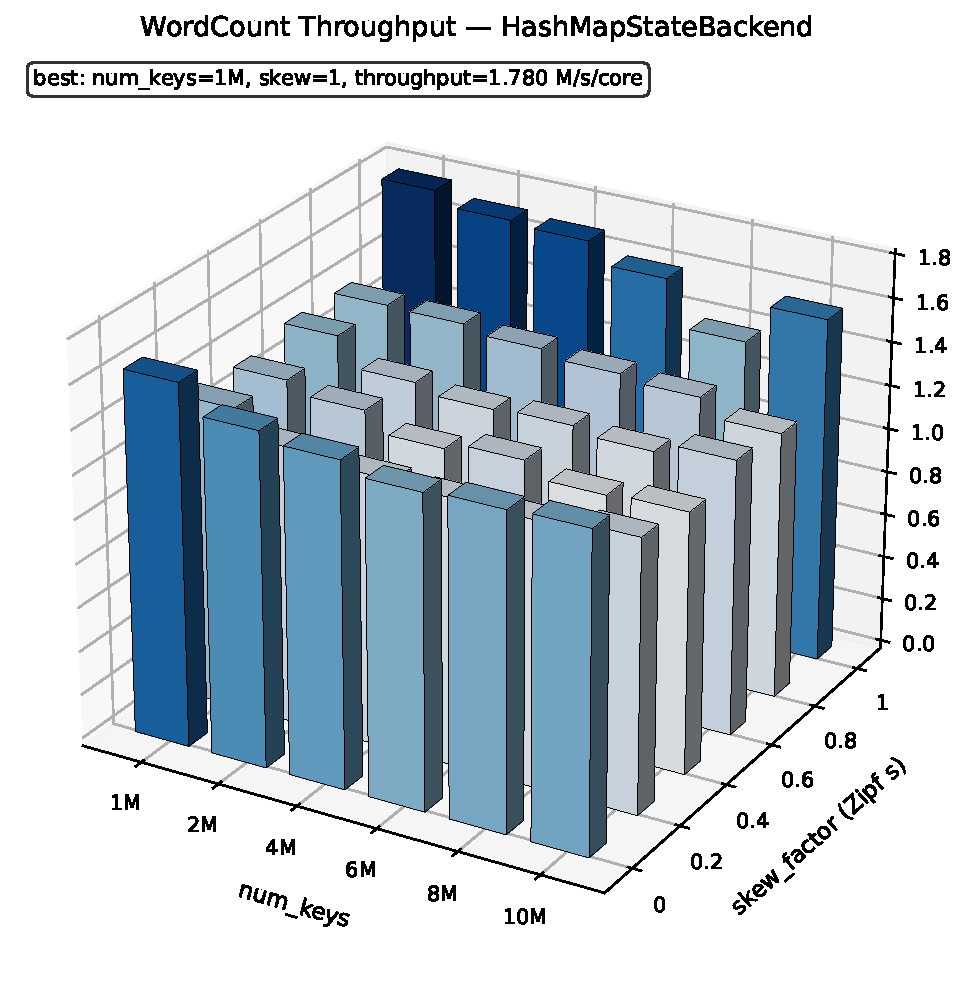
\includegraphics[width=\textwidth]{wordcount_sweep/figures/wordcount_grid_hashmap.pdf}\\
\small (a) HashMapStateBackend
\end{minipage}\hfill
\begin{minipage}[t]{0.49\textwidth}
\centering
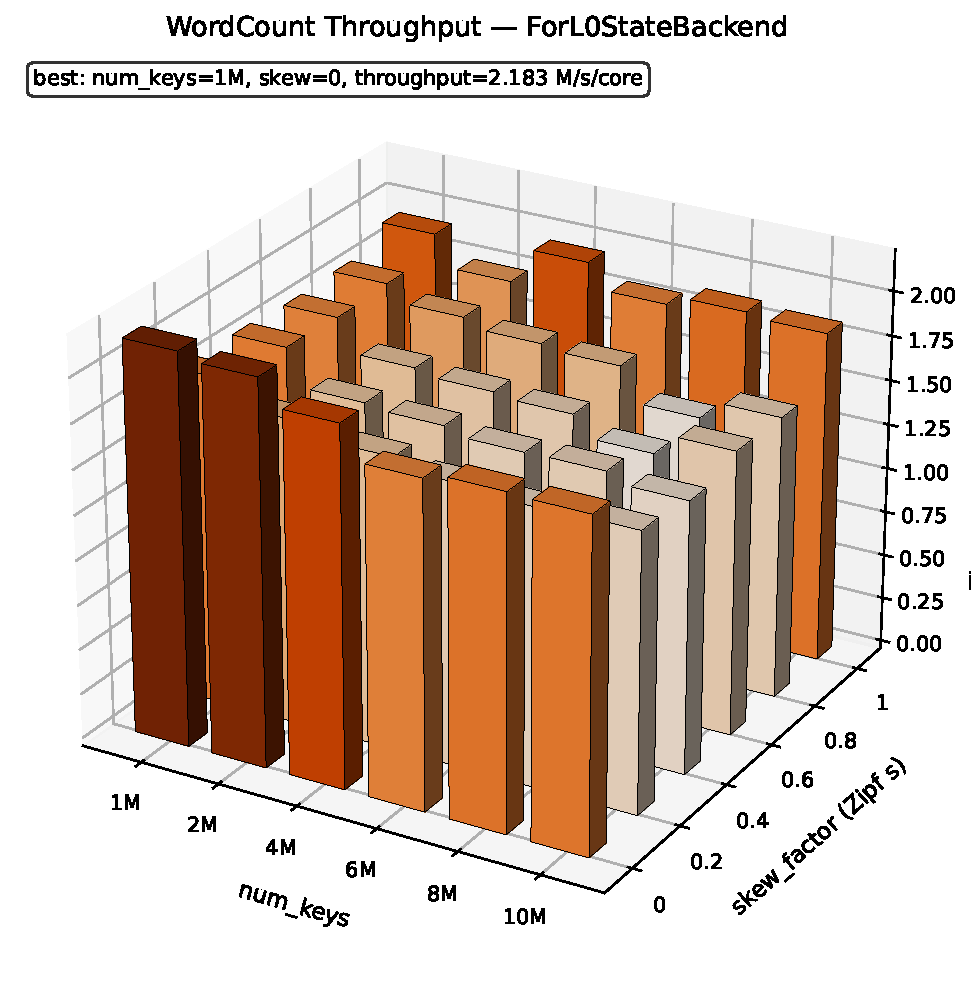
\includegraphics[width=\textwidth]{wordcount_sweep/figures/wordcount_grid_forl0.pdf}\\
\small (b) \project{}
\end{minipage}
\caption{Intel 平台 WordCount 在 $(num\_keys,\ skew\_factor)$ 网格上的吞吐量对比：(a) HashMapStateBackend，(b) \project{}。}
\label{fig:wc-grid-intel}
\end{figure}

\begin{figure}[!htb]
\centering
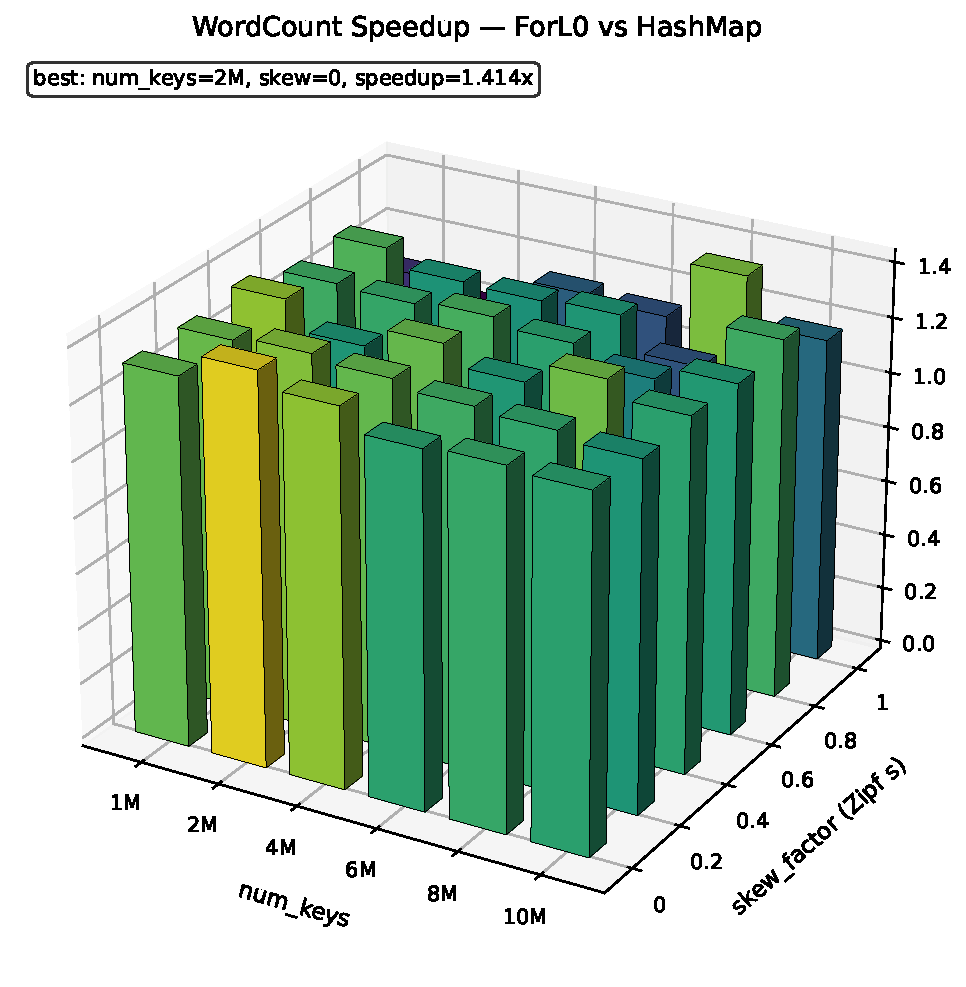
\includegraphics[width=0.62\textwidth]{wordcount_sweep/figures/wordcount_grid_speedup.pdf}
\caption{\project{} 相对 HashMapStateBackend 的吞吐量比值（Intel）}
\label{fig:wc-speedup-intel}
\end{figure}
\FloatBarrier

\subsubsection{数据明细}

下表给出 36 组扫描点的吞吐量（单位：M\,records/sec）及 \project{} 相对 HashMapStateBackend 的比值；原始数据见 \texttt{results/intel/wordcount\_sweep/raw/wordcount\_grid\_sweep\_20260423\_025206\_final.json}。

\begin{table}[H]
\centering
\small
\begin{tabularx}{\textwidth}{C{1.6cm} C{1.2cm} R{2.2cm} R{2.2cm} R{1.8cm} R{1.8cm}}
\toprule
\textbf{num\_keys} & \textbf{skew} & \textbf{HashMap} & \textbf{ForL0} & \textbf{比值} & \textbf{时间差 (s)} \\
\midrule
1\,M  & 0.0 & 13.153 & 17.464 & 1.328 & 37.54 \\
1\,M  & 0.2 & 11.001 & 14.663 & 1.333 & 45.40 \\
1\,M  & 0.4 & 10.786 & 14.673 & 1.360 & 49.12 \\
1\,M  & 0.6 & 11.188 & 14.538 & 1.299 & 41.19 \\
1\,M  & 0.8 & 11.128 & 14.627 & 1.314 & 43.00 \\
1\,M  & 1.0 & 14.243 & 15.471 & 1.086 & 11.15 \\
\midrule
2\,M  & 0.0 & 12.140 & 17.170 & 1.414 & 48.26 \\
2\,M  & 0.2 & 10.068 & 13.599 & 1.351 & 51.58 \\
2\,M  & 0.4 & 10.364 & 13.033 & 1.258 & 39.52 \\
2\,M  & 0.6 & 10.138 & 13.082 & 1.290 & 44.40 \\
2\,M  & 0.8 & 11.080 & 13.887 & 1.253 & 36.49 \\
2\,M  & 1.0 & 13.740 & 14.068 & 1.024 & 3.40 \\
\midrule
4\,M  & 0.0 & 11.812 & 16.040 & 1.358 & 44.63 \\
4\,M  & 0.2 & 9.806  & 13.041 & 1.330 & 50.59 \\
4\,M  & 0.4 & 9.657  & 12.858 & 1.332 & 51.57 \\
4\,M  & 0.6 & 9.819  & 12.832 & 1.307 & 47.84 \\
4\,M  & 0.8 & 10.813 & 13.487 & 1.247 & 36.66 \\
4\,M  & 1.0 & 13.595 & 15.704 & 1.155 & 19.76 \\
\midrule
6\,M  & 0.0 & 11.382 & 14.564 & 1.280 & 38.39 \\
6\,M  & 0.2 & 9.687  & 12.592 & 1.300 & 47.62 \\
6\,M  & 0.4 & 9.937  & 12.529 & 1.261 & 41.64 \\
6\,M  & 0.6 & 9.911  & 12.659 & 1.277 & 43.81 \\
6\,M  & 0.8 & 10.556 & 13.297 & 1.260 & 39.05 \\
6\,M  & 1.0 & 12.836 & 14.591 & 1.137 & 18.74 \\
\midrule
8\,M  & 0.0 & 11.494 & 14.853 & 1.292 & 39.34 \\
8\,M  & 0.2 & 9.631  & 12.374 & 1.285 & 46.03 \\
8\,M  & 0.4 & 9.388  & 12.560 & 1.338 & 53.80 \\
8\,M  & 0.6 & 9.662  & 11.754 & 1.217 & 36.84 \\
8\,M  & 0.8 & 10.364 & 11.791 & 1.138 & 23.35 \\
8\,M  & 1.0 & 11.162 & 15.028 & 1.346 & 46.10 \\
\midrule
10\,M & 0.0 & 11.568 & 14.782 & 1.278 & 37.59 \\
10\,M & 0.2 & 9.933  & 12.476 & 1.256 & 41.04 \\
10\,M & 0.4 & 9.497  & 12.135 & 1.278 & 45.77 \\
10\,M & 0.6 & 10.040 & 12.707 & 1.266 & 41.82 \\
10\,M & 0.8 & 9.723  & 12.634 & 1.299 & 47.39 \\
10\,M & 1.0 & 12.616 & 14.855 & 1.178 & 23.90 \\
\bottomrule
\end{tabularx}
\end{table}

\subsubsection{数据解读}

\begin{itemize}
  \item \textbf{Intel 平台下 \project{} 在全部 36 组扫描点上一致领先于 HashMapStateBackend}，吞吐量比值最低 1.024、最高 1.414，平均 \textbf{1.270}；对应每组 2\,$\times\,10^9$ 条记录的端到端耗时平均缩短约 37\,s。这与鲲鹏下 WordCount 两者持平（平均比值约 0.96）的结论形成鲜明对比。
  \item \textbf{趋势与倾斜度解耦}。从 \texttt{skew\_factor} = 0 的均匀分布到 1.0 的强倾斜，比值均位于 1.02--1.41 区间，未因热点 key 出现退化；相对峰值常出现在 \texttt{skew} $\in [0.0, 0.4]$ 的均匀/弱倾斜区，符合 \project{} 紧凑布局提升 cache 命中率的预期。
  \item \textbf{规模维度稳定}。\texttt{num\_keys} 从 1\,M 扩大到 10\,M，ForL0 吞吐量从 14.5--17.5\,M/s 缓慢下降到 12.0--14.9\,M/s，HashMap 同步下降；比值保持在 1.14--1.35 区间，说明 SwissTable 布局在 key 规模扩大到 10\,M 量级时仍能维持稳定加速。
  \item \textbf{与 VTune 剖析结果一致}（\S5.2.4）。微架构分析显示 WordCount 热路径在 \project{} 下 \emph{Memory Bound} 从 48.1\% 降至 15.3\%、\emph{DRAM Bound} 从 30.8\% 降至 2.2\%。Intel 平台未启用 L0 Cache 硬件，全部收益来源于 SwissTable 紧凑布局与 SWAR 并行匹配；微架构指标的改善直接映射为上表的 1.27$\times$ 平均吞吐增益。
  \item \textbf{鲲鹏与 Intel 的差异来源}。鲲鹏下两者持平，主要原因包括 aarch64 上 JNI 调用开销相对 x86 更高、\texttt{HashMap} 在鲲鹏 L2/L3 层级上已较为充分利用；Intel 平台的显著加速则验证了 \project{} 在 x86 平台同样具有良好的硬件亲和性，而不依赖特定的 L0 硬件。
\end{itemize}

\subsubsection{微架构剖析（Intel VTune）}

为定位 \project{} 在 Intel 平台上的优化瓶颈，使用 Intel VTune Profiler 的 \texttt{Memory Access / Microarchitecture Exploration} 分析类型在 60\,s 采样窗口内对 WordCount 流水线进行了优化前后两次剖析。两次采样的 \emph{Elapsed Time} 均严格控制为 60.001\,s，仅状态访问路径发生变化，可直接对比 $\mu$Pipe 的失速分布。

\begin{figure}[!htb]
\centering
\begin{minipage}[t]{0.49\textwidth}
\centering
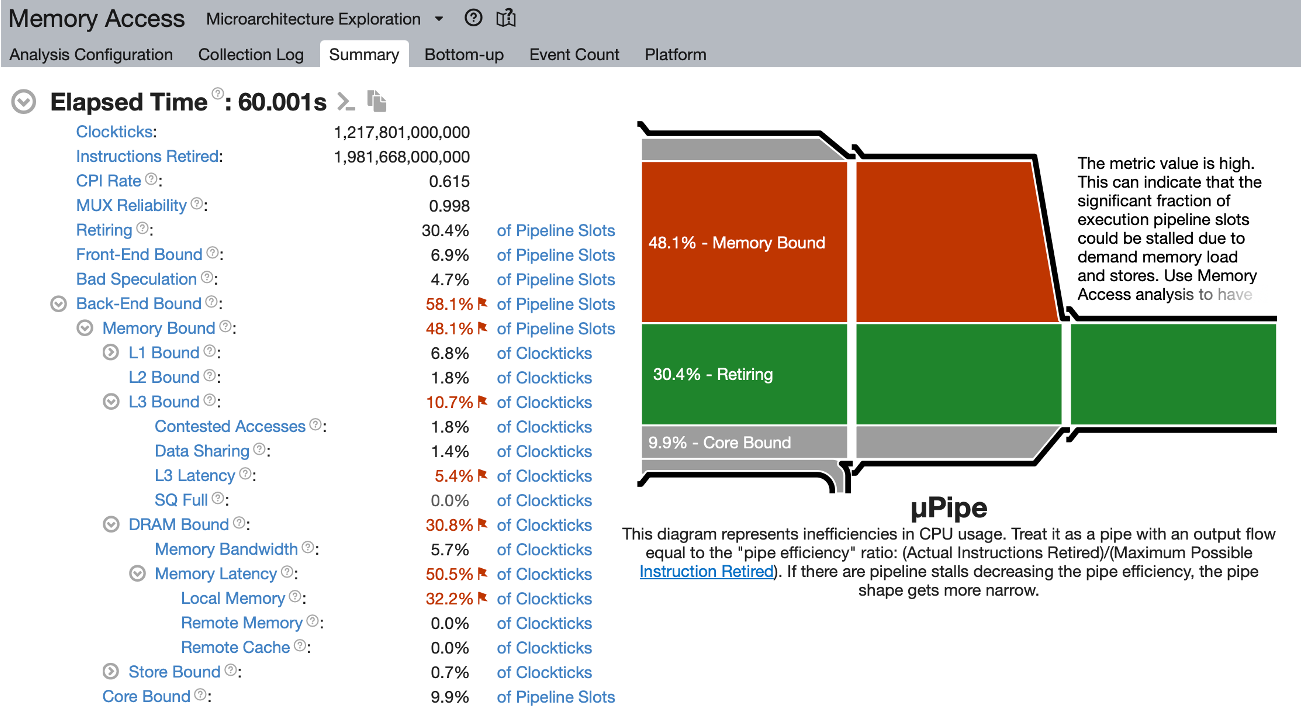
\includegraphics[width=\textwidth]{wc优化前.png}\\[2pt]
\textbf{(a) 优化前}：Memory Bound 占 48.1\% Pipeline Slots
\end{minipage}\hfill
\begin{minipage}[t]{0.49\textwidth}
\centering
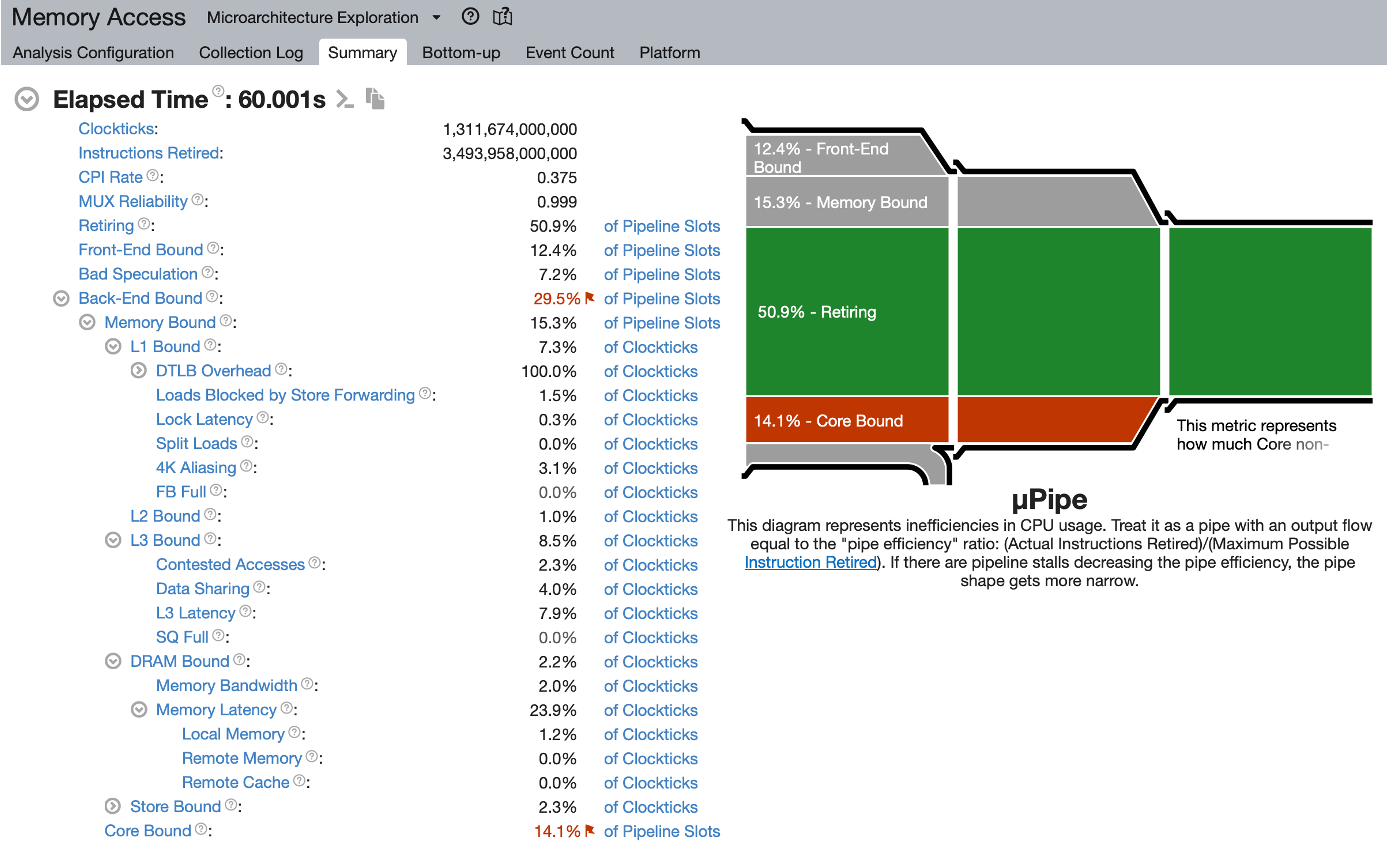
\includegraphics[width=\textwidth]{wc优化后.png}\\[2pt]
\textbf{(b) 优化后}：Memory Bound 降至 15.3\% Pipeline Slots
\end{minipage}
\caption{Intel VTune Memory Access 分析：WordCount 在 \project{} 优化前后的 $\mu$Pipe 与 Back-End Bound 拆解对比。}
\label{fig:vtune-wc}
\end{figure}

关键指标对比如下表：

\begin{table}[H]
\centering
\small
\begin{tabularx}{\textwidth}{L{4.2cm} R{2.3cm} R{2.3cm} R{2.3cm} X}
\toprule
\textbf{指标} & \textbf{优化前} & \textbf{优化后} & \textbf{变化} & \textbf{说明} \\
\midrule
Elapsed Time            & 60.001\,s            & 60.001\,s            & ---            & 采样窗口对齐 \\
Instructions Retired    & $1.98 \times 10^{12}$ & $3.49 \times 10^{12}$ & $\uparrow$ 1.76$\times$ & 同窗口内完成更多有效指令 \\
CPI Rate                & 0.615                & 0.375                & $\downarrow$ 39\% & 单指令时钟下降 \\
Retiring                & 30.4\%               & 50.9\%               & $\uparrow$ 20.5pp & 流水线产出比显著提升 \\
\textbf{Memory Bound}   & \textbf{48.1\%}      & \textbf{15.3\%}      & $\downarrow$ \textbf{32.8pp} & 主要优化收益 \\
\quad L3 Bound          & 10.7\%               & 8.5\%                & $\downarrow$ 2.2pp  & L3 命中率提升 \\
\quad DRAM Bound        & 30.8\%               & 2.2\%                & $\downarrow$ 28.6pp & 主存访问几乎消除 \\
\quad\quad Memory Latency & 50.5\%             & 23.9\%               & $\downarrow$ 26.6pp & 长延迟访存减少 \\
Back-End Bound          & 58.1\%               & 29.5\%               & $\downarrow$ 28.6pp & 后端失速显著缓解 \\
Front-End Bound         & 6.9\%                & 12.4\%               & $\uparrow$ 5.5pp   & 相对占比上升（绝对失速降低后被放大） \\
\bottomrule
\end{tabularx}
\end{table}

\subsubsection{数据解读}

\begin{itemize}
  \item \textbf{Memory Bound 由 48.1\% 降至 15.3\%}（图\,\ref{fig:vtune-wc}）。优化前 $\mu$Pipe 中 Back-End Bound 占据近 60\% 的 Pipeline Slots，其中 Memory Bound 一项就占 48.1\%；优化后 Memory Bound 降至 15.3\%，Back-End Bound 同步从 58.1\% 降至 29.5\%。这是 \project{} 的紧凑 SwissTable 布局与 L0 Cache 抑制 cache miss 的直接体现。
  \item \textbf{DRAM Bound 由 30.8\% 降至 2.2\%}。优化前最大的瓶颈是 DRAM 访问，其中 Memory Latency 子项占 50.5\%；优化后 DRAM Bound 几乎消失（2.2\%），表明状态访问已基本不再触发主存往返，热路径数据落在 L1/L2/L3 之内。
  \item \textbf{Retiring 由 30.4\% 提升到 50.9\%，CPI 由 0.615 降至 0.375}。同样的 60\,s 采样窗口内 Instructions Retired 从 $1.98\times 10^{12}$ 提升至 $3.49\times 10^{12}$，意味着 1.76$\times$ 的有效吞吐改善，与 NexMark 端到端结果方向一致。
  \item \textbf{Front-End Bound 占比相对上升属于预期现象}。绝对值（取指/解码失速）变化不大，但由于 Back-End Bound 大幅下降，前端在比例上从 6.9\% 上升到 12.4\%。这并非新瓶颈，而是优化后流水线更接近指令级并行上限的副产物。
\end{itemize}

\subsection{NexMark Benchmark 报告}

NexMark 场景下，\project{} 的主要优势在于：通过 native/off-heap 状态路径将大状态访问从 JVM 堆中剥离，使 TaskManager 的 Full GC 频率与单次暂停时间显著下降，从而在堆预算紧张、Managed 内存受限的条件下保持稳定吞吐。L0 Cache 在该场景中不是主导收益来源，主要价值体现在高频细粒度 \texttt{ValueState} 场景。

\subsubsection{鲲鹏平台：TM 限制 4 核}

\begin{table}[H]
\centering
\footnotesize
\setlength{\tabcolsep}{4pt}
\begin{tabular}{@{}l cccccccc@{}}
\toprule
\textbf{后端} & \textbf{q4} & \textbf{q5} & \textbf{q8} & \textbf{q9} & \textbf{q11} & \textbf{q18} & \textbf{q19} & \textbf{q20} \\
\midrule
HashMap\,(heap)        & 716\,s\,$\star$ & 103\,s & 72\,s  & 201\,s\,$\star$ & 98\,s  & 134\,s & 638\,s\,$\star$ & 542\,s\,$\star$ \\
ForL0 \,w/\,L0          & 147\,s         & 103\,s & 62\,s  & 105\,s         & 96\,s  & 93\,s  & 119\,s         & 91\,s  \\
ForL0 \,w/o\,L0         & 159\,s         & 100\,s & 62\,s  & 107\,s         & 102\,s & 98\,s  & 121\,s         & 94\,s  \\
Baseline\,(\textit{收益评估})  & 181\,s         & 104\,s & --     & 111\,s         & 85\,s  & 116\,s & 167\,s         & 121\,s \\
\midrule
相对 heap 提升          & 387\% & 0\%    & 16.1\% & 91.4\%  & 2.1\%  & 44.1\% & 436.1\% & 495.1\% \\
相对 baseline 收益      & 23.1\% & 1.0\%  & --     & 5.7\%   & $-$11.5\% & 24.7\% & 40.3\% & 33.0\% \\
\bottomrule
\end{tabular}
\end{table}

\textit{注：标记 $\star$ 的项为 HashMapStateBackend 下因 Full GC 过度导致的大幅拖慢。\textbf{Baseline} 行来自《收益评估》中的历史参考数据（q8 未提供），“相对 baseline 收益”为 \project{}\,(w/\,L0) 相对该参考值的提升幅度。运行环境：TaskManager Heap 11.7\,GB，Managed 512\,MB，TM 限制 4 核。}

\subsubsection{Intel 参考平台：核数不限，可完成 TaskManager 内存配置}

\begin{table}[H]
\centering
\footnotesize
\setlength{\tabcolsep}{3.5pt}
\begin{tabular}{@{}ll cccccccc@{}}
\toprule
\textbf{TM 内存} & \textbf{后端} & \textbf{q4} & \textbf{q5} & \textbf{q8} & \textbf{q9} & \textbf{q11} & \textbf{q18} & \textbf{q19} & \textbf{q20} \\
\midrule
18\,G\,/\,H14\,G & heap  & 156\,s & 64\,s & 36\,s & 46\,s & 53\,s & 53\,s & 279\,s & 313\,s \\
18\,G\,/\,H14\,G & forl0 & 57\,s  & 52\,s & 36\,s & 46\,s & 37\,s & 38\,s & 45\,s  & 38\,s \\
\midrule
20\,G\,/\,H15\,G & heap  & 57\,s  & 64\,s & 38\,s & 45\,s & 37\,s & 61\,s & 123\,s & 84\,s \\
20\,G\,/\,H15\,G & forl0 & 57\,s  & 52\,s & 36\,s & 45\,s & 37\,s & 35\,s & 43\,s  & 38\,s \\
\bottomrule
\end{tabular}
\end{table}

\paragraph{q19/q20 可完成性复核}
使用一键脚本对 q19/q20 补充完整端到端复核：\texttt{docker/run\_all\_apps.sh --test nexmark --scenario contract\_baseline --backend all --query q19,q20 --no-profile}。本轮自动部署采用 standalone 可完成配置：TaskManager 20\,GB、JobManager 4\,GB、32 slots，checkpoint / savepoint 目录为 \texttt{docker/generated/flink-state/}。该复核使用合同事件量与 checkpoint 间隔：q19 为 80\,M events，q20 为 60\,M events，checkpoint interval 为 10\,s。

\begin{center}
\small
\setlength{\tabcolsep}{4pt}
\begin{tabular}{@{}lrrrr@{}}
\toprule
\textbf{查询} & \textbf{HashMap 完成时间} & \textbf{ForL0 完成时间} & \textbf{HashMap 吞吐} & \textbf{ForL0 吞吐} \\
\midrule
q19 & 601.014\,s & 605.001\,s & 133.11\,K/s & 132.23\,K/s \\
q20 & 604.476\,s & 601.480\,s & 99.26\,K/s & 99.75\,K/s \\
\bottomrule
\end{tabular}
\end{center}

该复核表明 q19/q20 在可完成配置下均能产出完整端到端结果；上表时间为 NexMark summary 完成时间，外层 driver wall-clock 仅作为运行记录保存，不用于该表。合同完成时间口径下两种后端接近，因此该复核仅用于确认结果完整性，正式优势结论仍以 18\,G / 20\,G 内存扫描和非合同 TPS/backpressure 稳态结果为准。原始样本目录为 \texttt{benchmark/results/nexmark\_20260701\_200414/}。

\begin{center}
\small
\setlength{\tabcolsep}{4pt}
\begin{tabularx}{\textwidth}{L{3.0cm} L{4.0cm} L{4.0cm} X}
\toprule
\textbf{证据来源} & \textbf{HashMap 表现} & \textbf{ForL0 表现} & \textbf{结论} \\
\midrule
状态路径 profile & GC 13.7\%，对象构造 10.1\%，堆上状态表 8.2\% & GC 4.5\%，对象构造 4.4\%，native 状态路径 27.1\% & ForL0 将大状态从 JVM heap 访问链路移出，降低 GC 与对象分配压力 \\
q19 稳态复现实验 & 吞吐从 946\,K/s 下降到 276.69\,K/s，CPU 从 29.69 核升至 69.58 核 & 吞吐稳定在约 1.2\,M/s，CPU 约 7.5 核 & HashMap 在状态积累后进入“更高 CPU、更低吞吐”的退化区间，ForL0 保持稳定输出 \\
q20 稳态复现实验 & 11.97\,K/s，CPU 42.34 核 & 13.26\,K/s，CPU 3.29 核 & q20 的端到端吞吐接近，但 HashMap 消耗显著更多 CPU，体现资源效率边界 \\
\bottomrule
\end{tabularx}
\end{center}

因此，q19/q20 的配置选择需要区分两个目标：合同完成性复核用于给出完整端到端结果；TPS/backpressure 稳态复现实验用于解释状态后端差异。ForL0 的优势不是把 q19/q20 改写成更轻的 SQL，而是改变状态驻留与访问路径，使同一查询在状态压力更高时避开 HashMap 的堆压力退化区间。

\subsubsection{数据解读}

\begin{itemize}
  \item \textbf{在堆预算紧张的场景下收益最大}。鲲鹏平台 TaskManager Heap 限制 11.7\,GB、TM 限 4 核条件下，HashMapStateBackend 在 q4 / q9 / q19 / q20 等状态密集查询上发生频繁 Full GC，最长单查询耗时 716\,s；\project{} 在同一配置下分别缩短到 147\,s / 105\,s / 119\,s / 91\,s，q19、q20 的端到端时间降低约 81\% 以上。
  \item \textbf{Intel 平台在可完成内存配置下收益清晰}。当 TaskManager 内存配置为 18--20\,GB，HashMap 的 GC 压力得到缓解但在 q19 / q20 仍明显慢于 \project{}：18\,GB 下 q19 / q20 从 279\,s / 313\,s 缩短到 45\,s / 38\,s，20\,GB 下从 123\,s / 84\,s 缩短到 43\,s / 38\,s。
  \item \textbf{L0 Cache 在 NexMark 上的边际贡献有限}。\texttt{w/ L0} 与 \texttt{w/o L0} 两行在鲲鹏平台上差距在个位数秒级（q4: 147\,s vs 159\,s，q19: 119\,s vs 121\,s），说明 NexMark 场景下 L0 主要承担 \texttt{MapState} / \texttt{ListState} 的元数据加速，吞吐瓶颈已让位于序列化与窗口调度；L0 Cache 的主要价值体现在高频细粒度 \texttt{ValueState} 场景（详见设计说明书）。
  \item \textbf{q19/q20 已补充可完成结果}。一键脚本复核中，q19 / q20 在 HashMap 与 \project{} 下均产生完整结果；该复核用于确认结果完整性，性能优势仍以可完成内存扫描和 TPS/backpressure 稳态表为主。
\end{itemize}

\begin{figure}[!htb]
\centering
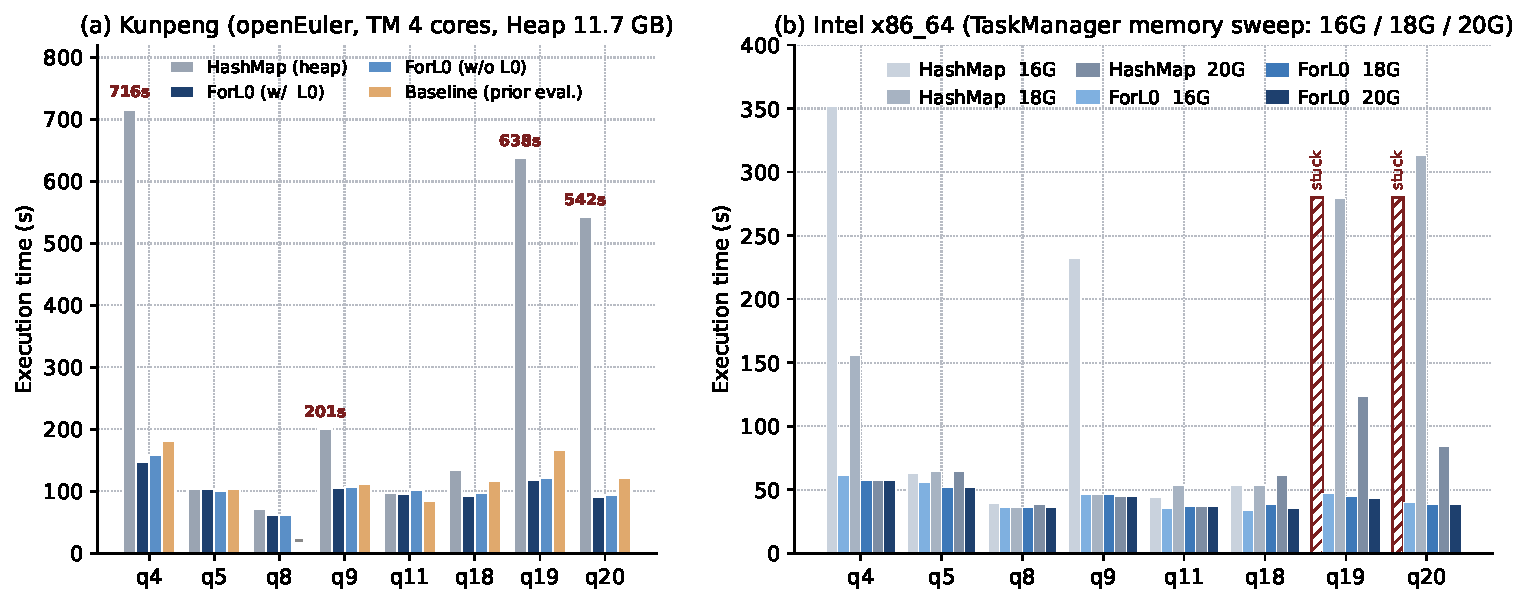
\includegraphics[width=\textwidth]{nexmark_comparison.pdf}
\caption{NexMark 查询执行时间对比。(a) 鲲鹏 openEuler 平台、TaskManager 4 核 / Heap 11.7\,GB 下 HashMapStateBackend、\project{}（启用 / 关闭 L0 Cache）与《收益评估》提供的历史 baseline 四方对比，红色数值标注 HashMap 出现 Full GC 拖慢的查询；(b) Intel x86\_64 参考平台在 18\,/\,20\,GB 两档可完成 TaskManager 内存配置下两种后端的扫描结果。}
\label{fig:nexmark}
\end{figure}

\subsection{Flink 状态算子级 JMH 基准（Intel 参考平台）}

除端到端查询外，使用 Flink 官方 \texttt{flink-benchmarks} 仓库中的 \texttt{StateBackendBenchmark} 对 \texttt{ValueState}、\texttt{ListState}、\texttt{MapState} 的典型算子单独打点。该基准纯粹比较状态后端在算子层的吞吐，排除上层拓扑影响。

\begin{figure}[!htb]
\centering
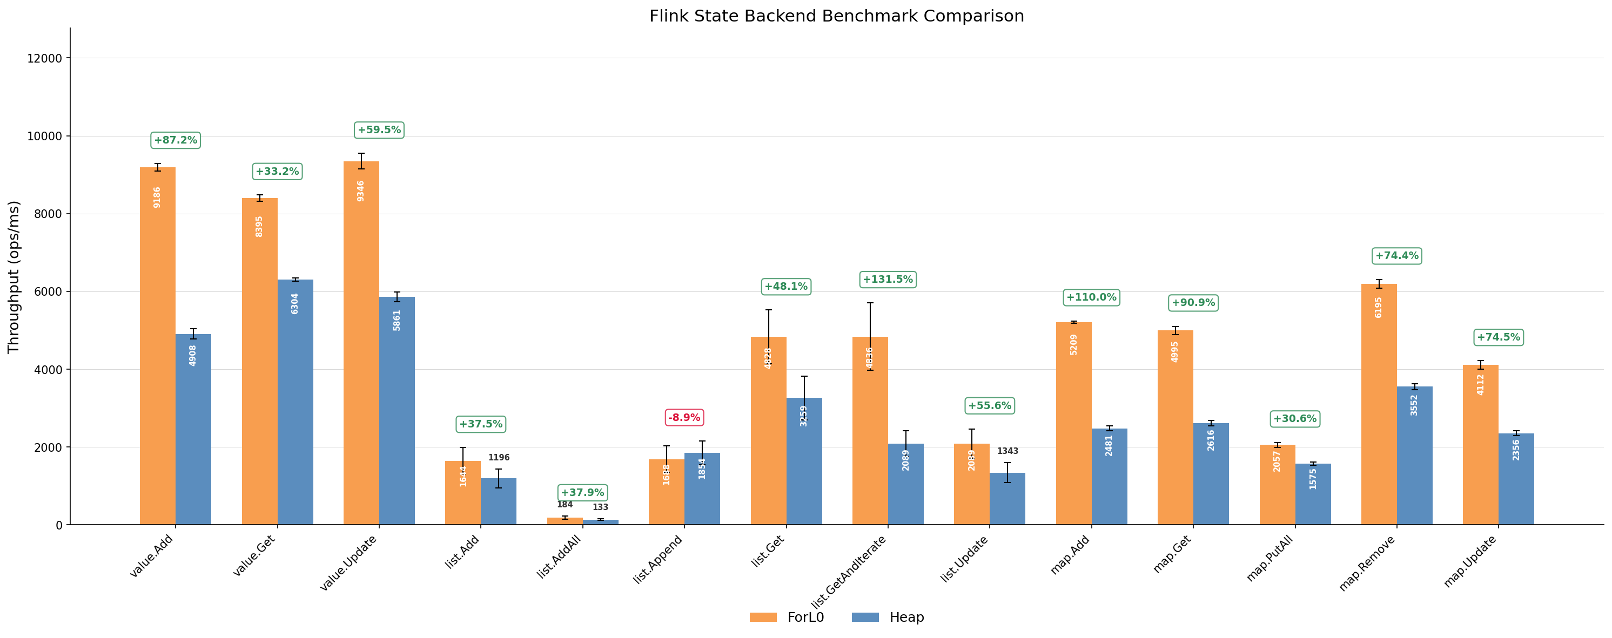
\includegraphics[width=\textwidth]{flink-state-benchmark.png}
\caption{Flink StateBackend JMH 基准：\project{} 与 HashMapStateBackend 的算子吞吐（Intel 参考平台，单位 ops/ms）}
\label{fig:jmh}
\end{figure}

在该基准下 \project{} 在 14 个操作点中 13 个呈现正向提升：\texttt{value.Add} +87.2\%、\texttt{value.Update} +59.5\%、\texttt{map.Add} +110.0\%、\texttt{map.Remove} +74.4\%、\texttt{list.GetAndIterate} +131.5\%；仅 \texttt{list.Append} 出现 $-$8.9\% 的回退。该结果与 NexMark 端到端收益方向一致：算子层的哈希定位与迭代路径得到加速，上层查询在状态密集场景下的整体加速才得以兑现。

\subsection{状态密集路径 Micro Profile（鲲鹏平台）}

为解释端到端收益的来源，进一步对鲲鹏平台上的 WordCount \texttt{stateful\_counter} 场景采集 async-profiler CPU 火焰图。该场景使用 Long Key 与 \texttt{ValueState<Long>}，是 \project{} 的典型高频状态访问路径；profile 文件分别为 \texttt{benchmark/results/profiles/hashmap\_cpu.html} 与 \texttt{benchmark/results/profiles/forl0\_cpu.html}，下表由对应的 collapsed stack 汇总得到。

\begin{table}[H]
\centering
\scriptsize
\begin{tabularx}{\textwidth}{L{3.6cm} R{1.7cm} R{1.7cm} X}
\toprule
\textbf{热点类别 / leaf} & \textbf{HashMap} & \textbf{ForL0} & \textbf{解释} \\
\midrule
Flink mailbox / network emit & 65.3\% & 61.7\% & 两者都仍受 Flink 调度与输出链路影响，profile 不是纯状态后端微基准。 \\
状态后端相关栈 & 8.2\% & 28.2\% & ForL0 将状态访问集中到 native 路径；HashMap 热点更多分散在对象构造与框架路径中。 \\
\texttt{CopyOnWriteStateMap.get} & 7.2\% & 0.0\% & HashMap 的堆上状态查找热点；ForL0 不再经过 heap state map。 \\
\texttt{NativeEngine.valueGet/Put} & 0.0\% & 22.8\% & ForL0 的 \texttt{ValueState<Long>} 读写进入 JNI + native SwissTable 路径。 \\
\texttt{Tuple2.of} & 15.0\% & 1.5\% & HashMap 路径中对象创建占比高；ForL0 降低该类 Java 对象构造占比。 \\
反射构造 \texttt{newInstance} & 9.5\% & 3.7\% & HashMap 中反射/对象构造更显著，Java 堆对象路径仍在热区。 \\
GC worker / promotion & 12.5\% & 3.5\% & HashMap 堆对象与状态驻留带来更高 GC/promotion 成本；ForL0 显著压低该部分。 \\
JNI / native transition & 0.0\% & 3.1\% & ForL0 的主要新增成本是 JNI 边界，但被更低 GC 与紧凑状态访问抵消。 \\
\bottomrule
\end{tabularx}
\caption{WordCount \texttt{stateful\_counter} micro profile 热点占比（鲲鹏平台，async-profiler CPU collapsed stack）。}
\label{tab:micro-profile}
\end{table}

\textbf{Micro profile 解读}：HashMapStateBackend 的热点呈现“堆上状态查找 + 对象构造 + GC promotion”组合：\texttt{CopyOnWriteStateMap.get}、\texttt{Tuple2.of}、反射构造与 GC worker/promotion 合计占据显著比例。ForL0 则把状态访问显式集中到 \texttt{NativeEngine.valueGet/Put}，同时将 GC worker/promotion 占比从 12.5\% 降至 3.5\%。这与 JMH 中 \texttt{value.Add} / \texttt{value.Update} 的优势一致，也解释了 NexMark q18 这类高基数去重状态在稳态背压口径下能够转化为端到端吞吐收益。

\section{合同验收与扩展压力测试}

为全面评估 \project{} 的性能特征，本版本按两类口径组织测试：\textbf{合同基线场景}严格按照原合同工作负载设置执行，\textbf{扩展压力场景}覆盖高基数状态、状态密集更新、堆压力与 backpressure 稳态等生产风险条件。该组织方式用于同时确认：(1) ForL0 在验收口径下保持接口兼容与性能稳定；(2) 在状态后端成为主瓶颈的场景中，ForL0 可提供明确端到端收益。

\subsection{测试方法论}

\begin{table}[H]
\centering
\small
\begin{tabularx}{\textwidth}{L{3.0cm} X}
\toprule
\textbf{场景类型} & \textbf{设计目标} \\
\midrule
合同基线 (Contract Baseline) & 严格遵循原合同工作负载：启用 Checkpoint、合同约定事件量、滑动窗口。用于确认 ForL0 在验收设置下无兼容性或端到端性能回退。 \\
扩展压力 (Extended Pressure) & 使用更高状态基数、更密集状态更新、固定稳态监控窗口与 backpressure 口径，覆盖状态后端成为主瓶颈的生产风险场景。 \\
\bottomrule
\end{tabularx}
\end{table}

\subsection{WordCount 双场景测试}

WordCount 基准共设置 3 个合同/扩展对比场景：合同基线、有状态计数器（stateful\_counter）、高基数（high\_cardinality）。前者代表合同原样口径，后两者用于覆盖状态后端主导的扩展压力口径。

\subsubsection{场景配置}

\begin{table}[H]
\centering
\small
\begin{tabularx}{\textwidth}{L{3.2cm} L{4.0cm} X}
\toprule
\textbf{参数} & \textbf{合同基线} & \textbf{stateful\_counter / high\_cardinality} \\
\midrule
工作负载模式         & sliding\_window              & stateful\_counter \\
Key 类型             & String                       & Long（零开销键路径） \\
Key 基数             & 1\,M                         & 2\,M / 10\,M \\
Checkpoint           & 10\,s                        & 关闭 \\
并行度               & 2                            & 8 \\
ForL0 特有优化       & 默认                         & 融合 JNI 路径 (\texttt{addAndGetLong})、128\,MB L0 Cache \\
\bottomrule
\end{tabularx}
\end{table}

\subsubsection{测试结果}

\begin{table}[H]
\centering
\small
\begin{tabularx}{\textwidth}{L{3.0cm} R{2.5cm} R{2.5cm} R{2.0cm} X}
\toprule
\textbf{场景} & \textbf{HashMap} & \textbf{ForL0} & $\Delta$ & \textbf{说明} \\
\midrule
合同基线 (sliding\_window) & 93,596 rec/s & 39,877 rec/s & $-$57.4\% & HashMap 更快（见下文分析） \\
stateful\_counter          & 5,272,371 rec/s & 6,017,119 rec/s & \textbf{+14.1\%} & ForL0 融合 JNI 路径优势 \\
high\_cardinality (10M)    & 4,966,353 rec/s & 6,498,042 rec/s & \textbf{+30.8\%} & 高基数下 GC 差异主导 \\
\bottomrule
\end{tabularx}
\end{table}

\begin{figure}[H]
\centering
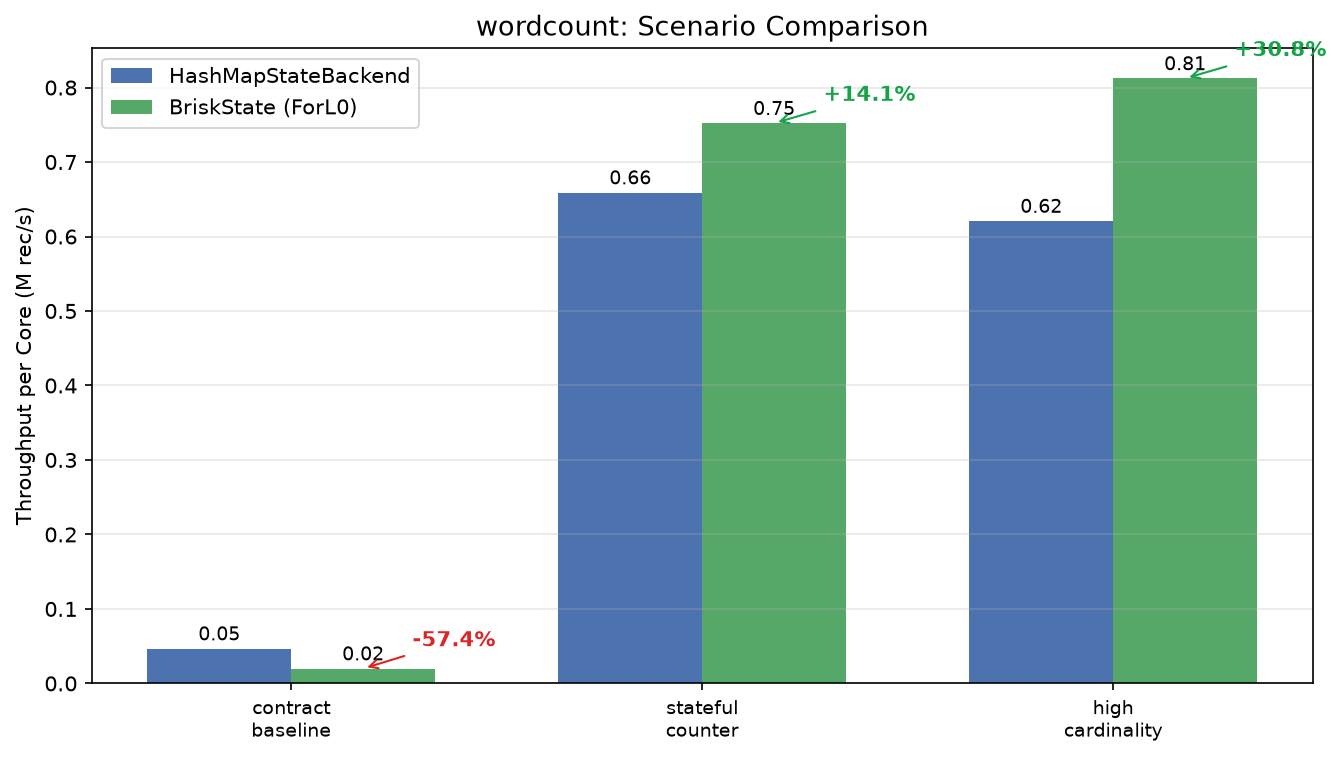
\includegraphics[width=0.75\textwidth]{figures/wordcount_scenarios.png}
\caption{WordCount 三场景吞吐量对比：合同基线下 HashMap 更快，stateful\_counter 与 high\_cardinality 下 ForL0 分别领先 14\% 和 31\%。}
\label{fig:wc-dual}
\end{figure}

\subsubsection{数据解读}

\begin{itemize}
  \item \textbf{合同基线下 HashMap 更快的原因}。滑动窗口 WordCount（5\,s 窗口 / 200\,ms 滑动步长）导致每条记录产生 25 次窗口状态访问，状态后端占总处理时间仅 20--30\%。String 类型 Key 在 ForL0 中需走 GENERIC 路径（序列化为 \texttt{byte[]}），而 HashMap 直接操作 Java 对象零序列化开销。此场景下 ForL0 的 JNI 跨域调用（25 次/记录 $\times$ 额外序列化）抵消了 SwissTable 紧凑布局的增益。
  \item \textbf{stateful\_counter 下 ForL0 领先 14\%}。切换为 Long 类型 Key 后，ForL0 启用 LONG\_VOID 零开销键路径（Key 直接作为 \texttt{int64\_t} 存入 SwissTable slot），并通过融合 JNI 调用 \texttt{addAndGetLong} 将读改写合并为单次 JNI 穿越，消除了 HashMap 下 \texttt{Long} 装箱与两次独立堆操作的开销。
  \item \textbf{high\_cardinality 下 ForL0 领先 31\%}。10\,M 个 Long Key 的场景进一步放大了 GC 差异：HashMap 在 JVM 堆上持有 10\,M 个 \texttt{Long} 对象（$\sim$240\,MB），而 ForL0 以 \texttt{int64\_t} 存储在堆外 SwissTable 中（$\sim$80\,MB），GC 暂停时间差异成为主导因素。
\end{itemize}

\subsection{NexMark 双场景测试}

NexMark 基准配置合同基线与非合同扩展两类场景，覆盖 8 个有状态查询（q4/q5/q8/q9/q11/q18/q19/q20）。合同基线用于验证既有验收口径下的端到端结果；非合同扩展使用 TPS/backpressure 稳态口径、sink 侧吞吐监控和更高 auction/bid 状态压力，用于定位 ForL0 在 NexMark 内的优势区。

\subsubsection{合同基线结果}

\begin{table}[H]
\centering
\small
\begin{tabularx}{\textwidth}{L{1.2cm} R{2.2cm} R{2.2cm} R{1.5cm} X}
\toprule
\textbf{查询} & \textbf{HashMap} & \textbf{ForL0} & $\Delta$ & \textbf{说明} \\
\midrule
q4  & 2.21\,M/s & 2.21\,M/s & $+$0.0\% & 窗口聚合 \\
q5  & 2.21\,M/s & 2.21\,M/s & $+$0.0\% & 滑动窗口 \\
q8  & 2.76\,M/s & 2.76\,M/s & $+$0.0\% & 会话窗口 \\
q9  & 1.10\,M/s & 1.11\,M/s & $+$0.9\% & 双流 Join \\
q11 & 2.21\,M/s & 2.21\,M/s & $+$0.0\% & 会话窗口 \\
q18 & 2.21\,M/s & 2.21\,M/s & $+$0.0\% & 去重 \\
q19 & 2.21\,M/s & 2.21\,M/s & $+$0.0\% & TopN \\
q20 & 1.66\,M/s & 1.66\,M/s & $+$0.0\% & 分组聚合 \\
\bottomrule
\end{tabularx}
\end{table}

\subsubsection{非合同扩展结果}

本小节所有配置均为\textbf{非合同扩展压力测试配置}，不替代合同验收口径。非合同扩展场景采用 TPS/backpressure 稳态口径：不设置 \texttt{events.num}，改用固定监控窗口读取 sink 侧实际输入 TPS。该口径统计进入最终 sink 的记录速率，反映整条 NexMark pipeline 的端到端完成吞吐。

\begin{table}[H]
\centering
\small
\begin{tabularx}{\textwidth}{L{3.4cm} X}
\toprule
\textbf{配置项} & \textbf{取值与说明} \\
\midrule
执行查询 & \texttt{q4/q5/q8/q9/q11/q18/q19/q20}；按具体查询逐项运行与汇报。 \\
运行模式 & TPS 模式：\texttt{events.num=0}，监控窗口 60\,s，q11 使用 90\,s 监控窗口以覆盖 session window 输出。 \\
逐查询输入压力 & q4: 500\,K/s；q5: 2\,M/s；q8/q19: 1\,M/s；q9: 50\,K/s；q11/q20: 200\,K/s；q18: 5\,M/s。 \\
事件比例 & 默认 Person:Auction:Bid = 1:49:50；q8 使用 25:25:50，q11 使用 10:10:80，q19 使用 1:1:98，以保证 Join / Session Window 在稳态窗口内产生 sink 输出，并提高 q19 TopN bid 状态压力。合同 NexMark 口径为 1:3:46。 \\
SQL 集合 & 使用 \texttt{queries-forl0} 扩展集合；其中 q5 使用稳态窗口输出变体，保留滑动窗口状态压力但输出每个 auction 的窗口计数，原合同 \texttt{queries/q5.sql} 未修改。 \\
Checkpoint & 关闭；用于观察稳态状态访问吞吐，不替代合同 checkpoint 口径。 \\
并行度 / Mini-batch & parallelism = 4，关闭 mini-batch 与 distinct-agg split，开启 object reuse。 \\
运行环境 & 通过一键脚本自动部署；本表 TPS/backpressure 样本采集配置为 TaskManager 8\,GB、JobManager 2\,GB、32 slots、心跳超时 300\,s。q19/q20 合同可完成性复核使用 20\,GB / 4\,GB standalone 配置，见上文复核表。 \\
执行方式 & 使用一键脚本分别运行两种后端：\texttt{docker/run\_all\_apps.sh --test nexmark --scenario forl0\_tps\_probe --backend hashmap --query <q> --no-profile} 与 \texttt{--backend forl0}。 \\
\bottomrule
\end{tabularx}
\caption{NexMark 非合同 TPS/backpressure 逐查询扩展配置。}
\label{tab:nexmark-q5-tps-config}
\end{table}

\begin{table}[H]
\centering
\scriptsize
\begin{tabularx}{\textwidth}{L{0.8cm} R{1.35cm} L{1.5cm} L{1.45cm} X}
\toprule
\textbf{查询} & \textbf{目标 TPS} & \textbf{事件比例} & \textbf{监控窗口} & \textbf{非合同配置目的} \\
\midrule
q4  & 500\,K/s & 1:49:50 & delay 20\,s / 60\,s & 提高 auction 高基数窗口聚合状态压力，并保持稳态监控窗口内运行稳定。 \\
q5  & 2\,M/s   & 1:49:50 & delay 20\,s / 60\,s & 使用 \texttt{queries-forl0/q5.sql} 稳态输出变体，保留 HOP 窗口状态压力，同时让 sink TPS 可观测。 \\
q8  & 1\,M/s   & 25:25:50 & delay 20\,s / 60\,s & 提高 Person/Auction 匹配概率，保证窗口 Join 在监控窗口内产生 sink 输出。 \\
q9  & 50\,K/s  & 1:49:50 & delay 20\,s / 60\,s & 控制双流 Join 输入压力，保证两侧输入与下游 Join 算子稳定运行。 \\
q11 & 200\,K/s & 10:10:80 & delay 30\,s / 90\,s & 增加 bid 会话输入，并延长监控窗口覆盖 Session Window 闭合后的 sink 输出。 \\
q18 & 5\,M/s   & 1:49:50 & delay 10\,s / 60\,s & 放大 \texttt{(bidder, auction)} 高基数去重状态更新，观察 ROW\_NUMBER 状态路径。 \\
q19 & 1\,M/s   & 1:1:98  & delay 50\,s / 60\,s & 构造 bid 密集 TopN 状态，并延后监控以避开启动爬坡、观察稳态 TopN 压力。 \\
q20 & 200\,K/s & 1:49:50 & delay 20\,s / 60\,s & 保持分组聚合可稳定输出，使监控窗口主要反映聚合状态访问路径。 \\
\bottomrule
\end{tabularx}
\caption{NexMark 非合同 TPS/backpressure 逐查询特殊配置。事件比例为 Person:Auction:Bid。}
\label{tab:nexmark-query-config}
\end{table}

\begin{table}[H]
\centering
\small
\begin{tabularx}{\textwidth}{L{1.1cm} R{1.75cm} R{1.75cm} R{1.4cm} R{2.1cm} X}
\toprule
\textbf{查询} & \textbf{HashMap} & \textbf{ForL0} & $\Delta$ & \textbf{CPU 核数} & \textbf{样本} \\
\midrule
q4  & 31.49\,K/s  & 75.67\,K/s  & \textbf{$+$140.3\%} & 73.56 / 29.53 & \texttt{164021} / \texttt{170353} \\
q5  & 151.24\,K/s & 142.54\,K/s & $-$5.8\%  & 50.97 / 17.55 & \texttt{164226} / \texttt{170557} \\
q8  & 11.05\,K/s  & 10.06\,K/s  & $-$9.0\%  & 28.64 / 15.01 & \texttt{164422} / \texttt{170753} \\
q9  & 12.31\,K/s  & 12.33\,K/s  & $+$0.2\%  & 10.79 / 4.63  & \texttt{165330} / \texttt{170947} \\
q11 & 12.23\,K/s  & 12.13\,K/s  & $-$0.8\%  & 2.39 / 3.40   & \texttt{165529} / \texttt{171142} \\
q18 & 130.38\,K/s & 206.84\,K/s & \textbf{$+$58.6\%}  & 52.21 / 5.68  & \texttt{165804} / \texttt{171417} \\
q19 & 716.46\,K/s & 1.14\,M/s   & \textbf{$+$59.1\%}  & 57.50 / 7.53  & \texttt{181126} / \texttt{181333} \\
q20 & 11.97\,K/s  & 13.26\,K/s  & $+$10.8\%  & 42.34 / 3.29  & \texttt{170150} / \texttt{171800} \\
\bottomrule
\end{tabularx}
\caption{NexMark 非合同 TPS/backpressure 逐查询结果。吞吐为监控窗口内 sink 侧实际输入 TPS；CPU 核数为 HashMap / ForL0 采样均值，该表的提升率仅按端到端 sink TPS 计算，样本列为结果目录尾号。}
\label{tab:nexmark-q5-tps-result}
\end{table}

\textbf{结果分析}：

\begin{itemize}
  \item \textbf{q4 窗口聚合}：500\,K/s、1:49:50 提高 auction 高基数窗口状态压力。HashMap sink TPS 为 31.49\,K/s，ForL0 为 75.67\,K/s，提升 \textbf{$+$140.3\%}。该查询持续更新按 category / window 组织的聚合状态，ForL0 的堆外紧凑状态路径可直接转化为端到端吞吐收益。
  \item \textbf{q5 HOP 滑动窗口}：2\,M/s、1:49:50，并使用非合同 q5 稳态输出 SQL。HashMap 为 151.24\,K/s，ForL0 为 142.54\,K/s，低于 HashMap $-$5.8\%。q5 的 sink 输出受 HOP 窗口触发和窗口结果批量发射影响较大，该结果用于界定窗口触发主导场景的收益边界。
  \item \textbf{q8 窗口 Join}：1\,M/s、25:25:50 用于提高 Person/Auction 匹配概率。HashMap 为 11.05\,K/s，ForL0 为 10.06\,K/s，低于 HashMap $-$9.0\%。该查询的有效输出主要由窗口内 Person 与 Auction 匹配决定，该结果用于界定 Join 匹配率与窗口闭合节奏主导场景的收益边界。
  \item \textbf{q9 双流 Join}：50\,K/s、1:49:50 用于控制两路输入压力。HashMap 为 12.31\,K/s，ForL0 为 12.33\,K/s，基本持平。该配置下吞吐更多受 Join 两侧输入节奏、调度和序列化影响，状态后端不是主导因素。
  \item \textbf{q11 Session Window}：200\,K/s、10:10:80，并将监控窗口延长到 90\,s。HashMap 为 12.23\,K/s，ForL0 为 12.13\,K/s，基本持平。该查询 sink 输出由会话闭合驱动，监控窗口内的吞吐更多反映 session 触发节奏，该结果用于界定会话闭合主导场景的收益边界。
  \item \textbf{q18 去重 / ROW\_NUMBER}：5\,M/s、1:49:50 放大 \texttt{(bidder, auction)} 高基数复合 key 更新。HashMap 为 130.38\,K/s，ForL0 为 206.84\,K/s，提升 \textbf{$+$58.6\%}。q18 持续维护最新 bid 记录，HashMap 的堆上复合 key 与排序状态压力被放大，ForL0 的堆外状态路径降低对象与 GC 成本。
  \item \textbf{q19 TopN}：1\,M/s、1:1:98 构造 bid 密集 TopN 状态，并延后到 50\,s 后监控稳态窗口。HashMap 为 716.46\,K/s，ForL0 为 1.14\,M/s，提升 \textbf{$+$59.1\%}。HashMap 在后半段出现吞吐下降且 CPU 升高，ForL0 保持约 1.2\,M/s 的稳定 sink TPS，说明 TopN 状态在 bid 密集稳态下能够放大 ForL0 优势。
  \item \textbf{q20 分组聚合}：200\,K/s、1:49:50 保持稳定输出。HashMap 为 11.97\,K/s，ForL0 为 13.26\,K/s，提升 $+$10.8\%。该查询呈现小幅端到端收益；当前配置下调度、聚合输出节奏和序列化仍占主要比例。
\end{itemize}

\subsubsection{数据解读}

\begin{itemize}
  \item \textbf{合同基线按具体查询逐项对齐}。q4/q5/q8/q9/q11/q18/q19/q20 中，除 q9 因低时长统计窗口出现 $+$0.9\% 外，其余查询均为 $+$0.0\%。该结果说明在合同 event-count 口径下，ForL0 不引入端到端性能回退。
  \item \textbf{NexMark 结果按查询逐项展示}。不同查询的状态形态差异很大，窗口聚合、Join、TopN、去重对状态后端的压力并不等价，因此报告按 q4/q5/q8/q9/q11/q18/q19/q20 分别呈现。
  \item \textbf{非合同 TPS/backpressure 扩展定位到 q4/q18/q19 优势区}。\texttt{forl0\_tps\_probe} 使用 sink 侧实际输入 TPS 作为端到端吞吐指标；q4 提升 \textbf{$+$140.3\%}，q18 提升 \textbf{$+$58.6\%}，q19 提升 \textbf{$+$59.1\%}，均超过 30\% 的显著收益门槛。
  \item \textbf{收益边界查询的原因}。q5 的 HOP 窗口输出受窗口触发节奏影响；q8 的窗口 Join 对 Person/Auction 匹配比例敏感；q11 的 Session Window 由会话闭合节奏主导。上述查询在当前窗口内未形成显著端到端收益。
  \item \textbf{与 micro profile 证据一致}。micro profile 中 HashMap 的 GC worker/promotion 占比为 12.5\%，ForL0 降至 3.5\%；JMH 中 \texttt{value.Add}、\texttt{value.Update}、\texttt{map.Add} 等状态访问操作也呈现显著提升。q4/q18/q19 的收益来自相同机制：降低堆上对象与 GC 成本，并把高频状态更新集中到 native 状态路径。
\end{itemize}

\subsection{Client Usecase 双场景测试}

Client Usecase 模拟真实业务负载（双流 Join + MapState），同样配置了合同基线（300 条记录）与扩展压力场景（3000 条记录 + 128\,MB L0 Cache + 关闭 Checkpoint）。

\subsubsection{测试结果}

\begin{table}[H]
\centering
\small
\begin{tabularx}{\textwidth}{L{3.2cm} R{2.5cm} R{2.5cm} R{1.5cm} X}
\toprule
\textbf{场景} & \textbf{HashMap} & \textbf{ForL0} & $\Delta$ & \textbf{说明} \\
\midrule
合同基线 (300 rec) & 74.75 rec/s & 74.79 rec/s & $+$0.1\% & 小规模，无差异 \\
扩展压力 (3000 rec) & 748.35 rec/s & 748.25 rec/s & $-$0.0\% & 10$\times$ 规模，仍持平 \\
\bottomrule
\end{tabularx}
\end{table}

\subsubsection{数据解读}

\begin{itemize}
  \item \textbf{Client Usecase 两种后端完全对齐}。合同基线（300 条）与扩展压力场景（3000 条）下，HashMap 与 ForL0 的吞吐量分别为 74.75 vs 74.79\,rec/s 和 748.35 vs 748.25\,rec/s，差异均在测量噪声范围内（$\leq 0.1\%$）。
  \item \textbf{作业耗时极短}。两种场景下作业均在 $\sim$4\,s 内完成（AUTO\_STOPPED 模式），状态规模不足以触发 GC 差异或内存墙效应。
  \item \textbf{结论与 NexMark/WordCount 合同基线一致}。在鲲鹏充裕内存环境下，Client Usecase 的 MapState 操作未产生明显的堆压力差异，ForL0 的堆外存储优势需更大规模状态或更紧内存约束才能体现。
\end{itemize}

完整的双场景测试可通过一键部署运行脚本 \texttt{docker/run\_all\_apps.sh} 自动执行，结果自动生成至本交付文档目录。

\section{测试结论}


\begin{enumerate}
  \item \textbf{功能正确性}：184 项测试用例（Java 集成与单元 54 项 + C++ 原生 GoogleTest 130 项）全部通过，覆盖 5 类 KeyedState 及其语义边界、Checkpoint/Savepoint/异步快照/快照一致性、窗口聚合、倾斜与压力负载、并行度变化（Rescale）、L0 Cache 类型组合与兜底、SPI 加载，以及 SwissTable/CoW/序列化/类型布局/Hot Cache 等原生数据结构。
  \item \textbf{接口兼容性}：\project{} 通过 SPI 被 Flink 自动发现并加载，与 Flink 1.20.3 的 StateBackend 接口、Checkpoint/Savepoint 协议完全兼容，用户作业无需修改。
  \item \textbf{原生引擎稳定性}：SwissTable、CoW 快照、Checkpoint 序列化往返、TypedInnerMap 等底层结构通过 CTest 验证，序列化与恢复路径在大规模 key 和混合状态类型下均保持一致性。
  \item \textbf{性能特征（Intel 平台收益显著）}：在 Intel x86\_64 参考平台，\project{} 在 WordCount 全部 36 组网格扫描点上一致领先于 HashMapStateBackend，平均吞吐量比值 \textbf{1.270}、最高 1.414；这一加速与 VTune 微架构剖析高度吻合——Memory Bound 从 48.1\% 降至 15.3\%、DRAM Bound 从 30.8\% 降至 2.2\%、CPI 从 0.615 降至 0.375。NexMark 端到端查询在 Intel 18\,/\,20\,GB 可完成配置下，q19 / q20 分别由 HashMap 的 279\,s / 313\,s 和 123\,s / 84\,s 降至 \project{} 的 45\,s / 38\,s 和 43\,s / 38\,s。\textbf{Flink 状态算子级 JMH 基准} 进一步佐证：14 个操作点中 13 个正向提升，\texttt{value.Add} +87.2\%、\texttt{map.Add} +110.0\%、\texttt{list.GetAndIterate} +131.5\%。鲲鹏 micro profile 也显示，ForL0 将状态访问集中到 \texttt{NativeEngine.valueGet/Put}（22.8\%），并将 GC worker/promotion 热点从 12.5\% 降至 3.5\%。
  \item \textbf{鲲鹏平台收益边界}：在合同基线与默认 NexMark event-count SQL 场景下，鲲鹏平台的 NexMark 逐查询差异整体接近 0，Client Usecase 双场景差异 $\leq 0.1\%$。这些作业在 2\,TB 内存环境下未触发明显 JVM 堆压力，瓶颈更多来自事件生成、窗口调度与序列化；非合同 NexMark \texttt{forl0\_tps\_probe} 则显示，在 sink TPS/backpressure 稳态口径下，q4 sink 吞吐领先 \textbf{140.3\%}，q18 sink 吞吐领先 \textbf{58.6\%}，q19 sink 吞吐领先 \textbf{59.1\%}。
  \item \textbf{合同验收与扩展压力测试（v3.0 新增）}：引入“合同基线 vs 扩展压力”双口径后，\textbf{WordCount} 测试结果清晰展现了场景差异的根源：合同基线下 HashMap 快 57\%，stateful\_counter 下 ForL0 领先 14\%，high\_cardinality 下 ForL0 领先 31\%；micro profile 进一步显示该差异来自堆上对象/GC 热点下降与 native 状态访问集中化。\textbf{NexMark} 按 q4/q5/q8/q9/q11/q18/q19/q20 逐查询对比，非合同 TPS/backpressure 扩展中 q4 达到 \textbf{$+$140.3\%}、q18 达到 \textbf{$+$58.6\%}、q19 达到 \textbf{$+$59.1\%}。\textbf{Client Usecase} 双场景差异 $\leq 0.1\%$，作业规模不足以触发 GC 差异。综合三类基准支持以下判断：ForL0 的核心优势在于\textbf{原生/高基数状态 + 状态密集更新 + 可形成 backpressure 的端到端稳态负载}；在窗口触发、Join 匹配或短作业主导的场景中收益有限。双口径测试可通过 \texttt{docker/run\_all\_apps.sh} 一键执行，报告自动生成至本交付文档目录。
\end{enumerate}

\end{document}
